\documentclass[useAMS,usenatbib]{mn2e}
\usepackage{myaasmacros}
\usepackage{graphicx}
\usepackage[normalem]{ulem}
\usepackage{amsmath}
\usepackage{multirow}
\usepackage{color}
\usepackage{amssymb}

\def\Glass{{\sc Glass}}
\def\PixeLens{{\sc PixeLens}}

\title[Light versus dark in strong-lens galaxies]{Light versus dark in strong-lens galaxies: Dark matter haloes that are rounder than their stars}

\author[Bruderer et al.]
{\parbox{\textwidth}{Claudio Bruderer,$^{1}$\thanks{E-mail: \texttt{claudio.bruderer@phys.ethz.ch}}
Justin I. Read,$^{1,2}$
Jonathan P. Coles,$^{3,4}$
Dominik Leier,$^{5}$
Emilio E. Falco,$^{6}$
Ignacio Ferreras$^{7}$ and
Prasenjit Saha$^{4,8}$}\vspace{0.4cm}\\
\parbox{\textwidth}{$^{1}$Institute for Astronomy, Department of Physics, ETH Zurich, Wolfgang-Pauli-Strasse 27, 8093 Z\"urich, Switzerland\\
$^{2}$Department of Physics, University of Surrey, Guildford, GU2 7XH, UK\\
$^{3}$Exascale Research Computing Lab, Campus Teratec, 2 Rue de la Piquetterie, 91680 Bruyeres-le-Chatel, France\\
$^{4}$Physik-Institut, University of Zurich, Winterthurerstrasse 190, 8057 Z\"urich, Switzerland\\
$^{5}$Dipartimento di Fisica e Astronomia, Universit\`{a} di Bologna, viale Berti Pichat 6/2, 40127, Bologna, Italy\\
$^{6}$Harvard-Smithsonian Center for Astrophysics, 60 Garden St., Cambridge, MA 02138, USA\\
$^{7}$Mullard Space Science Laboratory, University College London, Holmbury St Mary, Dorking, Surrey RH5 6NT, UK\\
$^{8}$Institute for Computational Science, University of Zurich, Winterthurerstrasse 190, 8057 Z\"urich, Switzerland}}


\begin{document}

\maketitle

\begin{abstract}
We measure the shape and alignment of the stellar and dark matter mass distribution in 11 strong-lens galaxies, finding over the range of several multiples of the half-light radii that the dark matter haloes are rounder than the stellar mass distributions. Averaging over larger radii, the ellipticity, as defined using the ratio of the semi-minor and semi-major axes, increases both in their dark matter and stellar components. While dark matter haloes are never more elliptical than $s_{dm} = 0.3$, their stars can extend to $s_* > 0.3$. Three systems, in particular, have a high stellar ellipticity ($s_* > 0.4$) and correspondingly a high alignment between the luminous and the dark matter distribution. One of these -- {\it B1608+656} -- is a known merging pair; we suggest that the other two ({\it B0712+472} and {\it B2016+112}) may also be recent post-merger systems. Galaxies with high dark matter ellipticity and weak external shear show strong alignment between light and dark; those with strong shear ($\gamma \gtrsim 0.1$) can be highly misaligned. This is reassuring since isolated misaligned galaxies are expected to be unstable.

Our results provide a new constraint on galaxy formation models that must explain the origin of both very round dark matter haloes and misaligned strong-lens systems.
\end{abstract}

\begin{keywords}
Gravitational lensing: strong -- galaxies: structure -- galaxies: haloes -- galaxies: formation -- galaxies: elliptical and lenticular, cD.
\end{keywords}


\section{Introduction}\label{sec:introduction}

The ellipticity and shape of the stellar component relative to their host dark matter halo encodes information both about our current cosmological model $\Lambda$CDM and galaxy formation \citep[e.g.][]{1994ApJ...431..617D,2001ApJ...551..294I,2004ApJ...611L..73K,2007MNRAS.378...55M,2007arXiv0707.0737D,2012MNRAS.424L..16L,2014JPhG...41f3101R}. `Dark-matter-only' (DMO) simulations in $\Lambda$CDM predict dark matter haloes that are triaxial \citep{1991ApJ...378..496D,1992ApJ...399..405W,1996ApJ...462..563N,2002ApJ...574..538J}, with mean `shape parameter' $\langle q \rangle = (b+c)/2a \sim 0.8$ (where $a > b > c$ are the long, intermediate and short axes of the figure; \citealt{2007MNRAS.378...55M}). This corresponds to a typically {\it prolate} halo. However, including `baryons' (stars and gas) in the models produces haloes that are significantly rounder and -- at least for disc galaxies -- well-aligned with the light distribution \citep{1991ApJ...377..365K,1994ApJ...431..617D,2007arXiv0707.0737D}. Halo shapes and alignments also constrain alternative gravity models \citep{2001MNRAS.327..552M,2004ApJ...610L..97H,2005MNRAS.361..971R,2012PhRvD..86h3507F,2013MNRAS.434.2971D}. If stars dominate the mass of the galaxy, we expect the light and mass distribution to be highly correlated; if dark matter is present, however, such correlations can, at least in principle, be broken.

Strong lensing provides a unique probe of the alignment and shape of the total mass distribution in galaxies \citep[e.g.][]{1986ApJ...310..568B,1992grle.book.....S,1998ApJ...509..561K,2000ApJ...543..131K,2006ApJ...649..599K,2007AJ....134..668A,2008MNRAS.383..857F,2010ApJ...724..511A,2012MNRAS.424..104L}. For `red and dead' ellipticals that are largely devoid of gas, their baryonic content can be mapped through stellar population synthesis modelling of their light distribution alone \citep[e.g.][]{2005ApJ...623L...5F,2006ApJ...640..662T,2008MNRAS.383..857F}. Furthermore, such systems are dense enough to produce strong lensing effects, opening up the possibility of directly comparing the light and mass in these galaxies \citep{1998ApJ...509..561K,2008MNRAS.383..857F,2009ApJ...690..670T,2012A&A...538A..99S}. Previous work in the literature has found that the light and mass are well-aligned (though a mis-match of up to 10$^\circ$ is not uncommon; e.g. \citealt{2012A&A...538A..99S}). However, results on the ellipticity of light and mass agree less well, with \citet{2012A&A...538A..99S} finding a strong correlation and \citet{1998ApJ...509..561K} and \citet{2008MNRAS.383..857F} finding none. It is difficult, however, to compare the results between these different studies because they use different lens modelling techniques; different definitions of ellipticity; and different radii over which the shapes and alignments are probed. Furthermore, none to date have applied their methodology to mock data to determine the robustness of the results.

Weak lensing can also be used to probe the shape and alignment between the luminous and dark matter distributions within galaxies. These galaxies however need to be `stacked' \citep{2000astro.ph..6281B,2000ApJ...538L.113N}, typically by aligning the major axes of the light distribution \citep[e.g.][]{2004ApJ...606...67H}. Given an elliptical total mass distribution, the exerted shear is larger in the direction of the major axis of the distribution than in the direction of the minor axis for fixed radii $r$ from the galaxy's center. In case of alignment of the luminous and dark matter and an elliptical shape of the distribution of the latter, the azimuthal distribution of this signal is thus expected to be anisotropic in absence of contaminating effects \citep[e.g. intrinsic alignments][]{2004PhRvD..70f3526H} and systematic effects. If the distributions are however misaligned or the mass distributions are spherical, the shear signal is expected to be isotropic.

This measurement has been perfomed on data by various groups \citep[][]{2004ApJ...606...67H,2006MNRAS.370.1008M,2007ApJ...669...21P,2012A&A...545A..71V} with inconclusive results. The analyses differ mainly in the data sets, the selection of lens galaxies, the estimators employed, and the treatment of systematics \citep[see][]{2015arXiv150704301S}. Recently, \citet{2015arXiv150603536C} made this measurement on Luminous Red Galaxies (LRG) in the Sloan Digital Sky Survey (SDSS), and report a significant detection of dark matter halo ellipticity. Shortly thereafter, \citet{2015arXiv150704301S} performed this measurement on blue and red galaxies in general identified in data from the Canada France Hawaii Lensing Survey (CFHTLenS), without being able to report a definite detection of halo ellipticity. However, their method was tested using the Milennium Simulation \citep{2005Natur.435..629S}, while exploring the effect of cosmic shear and misalignments of the luminous and dark matter distributions. This allows one to understand and predict the expected signal.
% \citet{2004ApJ...606...67H} applied this idea to data from the Red-Sequence Cluster Survey (RCS) to measure the first weak lensing signal of halo flattening. They found that dark matter haloes appear to be rounder than the stellar mass distribution, with some weak evidence for alignment. Both measurements are challenging however, and more recent data appear to be at odds with this early work, at least for galaxies in general. They however are in agreement concerning `red' galaxies, which are predominantly early-type galaxies, also favouring dark matter haloes that are more elliptical than their stellar mass components \citep{2006MNRAS.370.1008M,2007ApJ...669...21P,2012A&A...545A..71V}.}

% \citet{2004ApJ...606...67H}: Red-Sequence Cluster Survey (RCS); No split of galaxy sample in red & blue (magnitude-selected); Not taking care of systematics; f=0.77 --> probably good alignment, maybe halos somewhat rounder
% \citet{2006MNRAS.370.1008M}: Sloan-Digital Sky Survey (SDSS); Galaxy sample split based on color; Discussing systematics; f=0.10+-0.06; no definite detection of halo ellipticity
% \citet{2007ApJ...669...21P}: CFHTLS; No split of sample (rather only test by selecting preferentially ellipticals) (magnitude-selected); not really taking care of systematics, only test; halo ellipticity ~0.3 at 2sigma level (more if ellipticals)
% \citet{2012A&A...545A..71V}: Red-Sequence Cluster Survey (RCS2); split in red & blue (magnitude-selected); Discussing systematics; no definite detection of halo ellipticity
% \citet{2015arXiv150603536C}: SDSS; LRGs; Discuss systematics; detect halo ellipticity
% \citet{2015arXiv150704301S}: CFHTLenS; split in red & blue (magnitude-selected); Discussing systematics; no definite detection of halo ellipticity

Recently, \citet{2014MNRAS.445.2181C} introduced a new non-parametric lens tool, \Glass. Applying this to a large suite of mock data, we showed that mass and light can only reliably be disentangled in lens systems if: i) there are at least four images; and ii) time delay data are available and/or the stellar mass contributes significantly to the potential. In this paper, we collate data of the above quality, compiling a sample of 11 strong lens galaxies. We apply \Glass\ to these lenses to non-parametrically measure the shape and alignment of the stars and {\it dark matter} in these lens galaxies, for the first time. This differs from previous works that have all compared the light distribution with the total mass, rather than the dark matter. Since the stellar component often dominates the central potential, the total mass naturally correlates with the light, potentially masking theoretically interesting results about the dark matter distribution. Our comparison between the stellar and dark matter components is made possible by the fact that \Glass\ uses the stellar mass distribution as a prior on the mass map, ensuring that the dark matter map is always positive.

This paper is organised as follows. In Section~\ref{sec:shapemethod}, we briefly review the \Glass\ code and define our method to assess shape and alignment of lens galaxies. In Section~\ref{sec:data}, we present our data compilation with references. In Section~\ref{sec:results}, we present our results. Finally, in Section~\ref{sec:conclusions} we discuss the implications of these results and we present our main conclusions.


\section{The lens models}\label{sec:shapemethod}

While it is possible to compute shape parameters for a lensing galaxy by fitting to a parametric shape to the lens, it would make the definition of a shape estimate dependent on the which parametric form was being used. Moreover, the commonly-used parametric forms for modelling lensing galaxies \citep[e.g.][]{2001astro.ph..2341K} do not allow for features like twisting isodensity contours, which can arise from projection of triaxial ellipsoids with no intrinsic twists \citep[e.g.][and references therein]{1978ComAp...8...27B}. To avoid these problems, we use non-parametric ellipticity estimators, defined as follows.

Lenses are modelled as free-form mass distributions, consisting of mass tiles or pixels. Such lens models are also called non-parametric, which really just means that many more parameters than data constraints are used. Thus the lens models are non-unique, and hence in fact ensembles of these free-form mass distributions are used. From such a mass map, an inertia tensor is defined as
\begin{equation}\label{eq:inertiatensor}
I = 
\begin{pmatrix}
 \sum_\theta M(\boldsymbol{\theta})\theta^{2}_{y} & -\sum_\theta M(\boldsymbol{\theta})\theta_{x}\theta_{y} \\
-\sum_\theta M(\boldsymbol{\theta})\theta_{x}\theta_{y} & \sum_\theta M(\boldsymbol{\theta})\theta^{2}_{x}
\end{pmatrix}
\end{equation}
where the sum is over mass pixels, and $M(\boldsymbol{\theta})$ is the mass in a pixel. The eigenvectors of this inertia tensor give the ellipticity axes, and our ellipticity estimator is
\begin{equation}\label{eq:shapeestimate}
    s \equiv 1 - \frac{\lambda_{2}}{\lambda_{1}},
\end{equation}
where $\lambda_{1}$ and $\lambda_{2}$ ($\lambda_{1} \geq \lambda_{2}$) are the eigenvalues. We use this ellipticity estimators to quantify the shapes both of the stellar-mass distribution and of the dark-matter distribution. For the dark matter, only the mass distribution out to the radius of the outermost image is used; for the stellar part, the distribution with within different multiples of $R_e$ (defined as the half-light radius measured with respect to the Petrosian flux) is used. It is necessary to have a cutoff for the regions used to compute the inertia tensor, or else it would be dominated by the outer regions where there is little information \textbf{[CLAUDIO: Actually, I estimate the shapes for the luminous and dark matter in the same way. I only consider different Petrosian radii in Figure 3, setting different multiples of $R_e$ as a limit for both distributions. Figure 3 gives a sense of how much the estimates change if the distributions are analyzed only within a certain region...]}. The mass pixels used in this work are larger than image pixels, but at most 4\% of the diameter of the the full mass map. The central region has smaller pixels, to allow for a density cusp at the centre.

We estimate the orientation of the distributions of luminous and dark matter by computing the angles $\theta_{*}$ resp. $\theta_{dm}$ of the eigenvector corresponding to the eigenvalue $\lambda_{1}$ ($\lambda_{1} \geq \lambda_{2}$) relative to the x-axis. The misalignment angle $\Delta\theta$ between the distributions is then defined as
\begin{equation}
  \Delta\theta = \theta_{dm} - \theta_{*}.
\end{equation}

Each model ensemble consists of $10^4$ models, for all of which we apply our estimators for the shape and the alignment of the distributions. By identifying the median value and the range 68\% of all the values lie within of this distribution of estimated values, these quantities are constrained and the statistical uncertainties estimated.

The non-parametric mass models themselves are constructed using the \Glass\ framework for modelling multiple-image lenses \citep{2014MNRAS.445.2181C}. \Glass\ produces ensembles of mass maps, each of which reproduces exactly the observed image positions and image parities; also time delays, if measured. The lensing data must be in the form of point images, which could be quasars or simply point-like features in otherwise extended images, but this was not a problem for the lenses studied in this work. The estimated stellar mass (explained below in Section~\ref{sec:data}) is taken as a lower limit on the total mass. The additional mass that needs to be put on top, in order to reproduce the lensing observables, is interpreted as dark matter. \textbf{(Some of that mass may actually be gas, but very little is expected in the early-type galaxies used in this work.) [IS THIS SUPPOSED TO BE IN HERE?]} The criteria of lensing observables and non-negative dark matter by themselves would leave the mass distribution too under-determined. Hence, an additional prior is used, requiring the mass distribution to be centrally concentrated, with the same centre as the galaxy light (but not necessarily the shape). The precise formulation of the prior is given in Section~3 of \citet{2014MNRAS.445.2181C}.\footnote{Alternatively, see \citep{2015MNRAS.447.2170K} for a more intuitive account of \Glass.  Section~3.2 therein summarises the prior.} Tests of how well the shape estimator can be recovered from lensing data are given in Section~5.2 and Figure~8 of that paper.

\Glass\ is closely related to an earlier code \PixeLens\ \citep{2004AJ....127.2604S,2008ApJ...679...17C}, but has a completely different code base. An important improvement is a better sampling algorithm for high dimensional spaces \citep{2012MNRAS.425.3077L} that eliminates the excessive weight \PixeLens\ tended to give to extreme models.

\section{Data}\label{sec:data}
\begin{table}
  \begin{center}
    \begin{tabular}{l r r r r l}
      Lens & \multicolumn{1}{c}{$z_{L}$} & \multicolumn{1}{c}{$z_{S}$} & \multicolumn{1}{c}{$\Delta\theta$ [kpc]} & \multicolumn{1}{c}{$R_{L}$/$R_{e}$} & Environment \\ \hline
      0047 & 0.485 & 3.60 & 12.82 & $1.45\pm0.04$ & G(9) \\
      0414 & 0.960 & 2.64 & 16.01 & $1.85\pm0.05$ & ... \\
      0712 & 0.410 & 1.34 & 6.82  & $1.15\pm0.03$ & ... \\
      0911 & 0.769 & 2.8  & 23.16 & $3.09\pm0.05$ & C \\
      0957 & 0.356 & 1.41 & 29.98 & $3.51\pm0.04$ & C \\
      1115 & 0.310 & 1.72 & 10.76 & $2.86\pm0.06$ & G(13) \\
      1422 & 0.337 & 3.62 & 6.02  & $4.49\pm0.06$ & G(17) \\
      1608 & 0.630 & 1.39 & 13.92 & $1.82\pm0.01$ & G(8) \\
      2016 & 1.010 & 3.3  & 26.22 & $6.12\pm0.14$ & C(69) \\
      2045 & 0.870 & 1.28 & 14.46 & $1.48\pm0.03$ & ... \\
      2237 & 0.039 & 1.7  & 1.40  & $0.89\pm0.01$ & ... \\
    \end{tabular}
    \caption[width=\linewidth]{The most relevant lens properties for this work are listed \citep[for an expanded version of this table see][]{2011ApJ...740...97L}. References can be found in Section~\ref{sec:data}. The columns are from left to right: the lens redshift $z_L$; the redshift of the source $z_S$; the maximum angular separation between two images $\Delta\theta$; the ratio of the radius of the outermost image $R_L$ and the effective Petrosian half-light radius of the lens $R_e$; and information on the environment of the lens. C and G denote a known cluster or group environment, respecitvely. The number in the brackets is the number of confirmed members. Ellipses indicate lens galaxies with no group members identified so far.}
    \label{tab:lensproperties}
  \end{center}
\end{table}

\begin{table}
  \begin{center} \begin{tabular}{l l l l}
      Lens & Time delays [days] & Symmetric? & Comments \\ \hline
      0047 &  & \\
      0414 &  & \\
      0712 &  & \\
      0911 & $\Delta t_{BA}=146^{+4}_{-4}$ & yes\\
      0957 & $\Delta t_{BA}=416.5^{+1}_{-1}$ & yes \\
      1115 & $\Delta t_{BA}=12.0^{+2}_{-2}$ & \\
           & $\Delta t_{DC}=4.4^{+3.2}_{-2.4}$ & \\
      1422 &  & yes \\
      1608 & $\Delta t_{BA}=31.5^{+2}_{-1}$ & \\
           & $\Delta t_{CA}=36.0^{+1.5}_{-1.5}$ & \\
           & $\Delta t_{DA}=77.0^{+2}_{-1}$ & \\
      2016 &  & & Smaller pixels \\
      2045 &  & yes & $\gamma\leq 0.1$ \\
      2237 &  & \\
    \end{tabular}
    \caption[width=\linewidth]{Lenses where additional data or priors were used (cf.~Section~\ref{sec:shapemethod}). $\Delta t_{BA}$ and so on denote time delays between images as labelled in Table~\ref{tab:lenspositions}; $\gamma$ refers to the allowed external shear; Symmetric `yes' means the mass map is symmetric under rotation by $180^\circ$; `Smaller pixels' indicates that the mass pixels are 3\% (rather than 4\%) of the diameter of the whole mass map.}
    \label{tab:lenspriors}
  \end{center}
\end{table}

Stellar mass maps are taken from \citet{2011ApJ...740...97L}. In that work, the surface brightness distribution of the galaxy images in all available HST bands was first fitted using {\sc Galfit v2.03b} \citep{2002AJ....124..266P}, and with the resulting flux maps stellar mass maps using the synthesis of the stellar-population (SPS) models of \citet{2003MNRAS.344.1000B} were obtained. The population synthesis is marginalised over the star formation epoch and time scales and over the stellar metallicity. The initial mass function (IMF) was taken to be the log-normal form given by \citet{2003PASP..115..763C}; a more bottom-heavy IMF would change the mass normalisation \citep[cf.][]{2014ApJ...793...96S} but not the shape of the inferred stellar mass distribution \citep[unless the IMF presents significant intrinsic deviations locally, see e.g.][]{2015MNRAS.447.1033M}. We note that the effect of recent claims towards a non-universal IMF on stellar mass-to-light ratio (M/L) is still under debate. While for massive elliptical galaxies, dynamical studies seem to point at contributions at the level of the Salpeter IMF or slightly heavier \citep{2013MNRAS.432.1862C}, spectral line strength constraints can still accommodate a wider range of the stellar M/L depending on the functional form of the IMF \citep{2013MNRAS.429L..15F}. For at least one lens in our sample, \textit{Q2237+030}, the lensing estimates on the mass distribution are inconsistent with a Salpeter IMF \citep{2010MNRAS.409L..30F}. We additionally tested varying the IMF for one lens ({\it B1422+231}), finding that Salpeter IMF is too heavy and gives no solutions. We will perform a more systematic study of the IMF and varying stellar M/L in a forthcoming publication.

The original sample we consider, is presented in \citet{2011ApJ...740...97L} and consists of 21 lens systems. It is a subsample of the CfA-Arizona Space Telescope LEns Survey\footnote{http://www.cfa.harvard.edu/castles/} (CASTLES) sample. As shown in \citet{2014MNRAS.445.2181C}, the recovery of the shape information of the lens is only good if there are at least four images. Therefore, we only consider the quad lenses and the twin double \textit{Q0957+561}. This yields a sample consisting of 11 lenses. We discuss each of these systems, next. We note that all the position angles are measured north through east and relative to the lens galaxy.

\textit{Q0047-2808} (hereafter \textit{0047}) is a luminous early-type galaxy \citep{1996MNRAS.278..139W}. It is part of a group of 9 members, all of which are spectroscopically confirmed \citep{2011ApJ...726...84W}.

\textit{MG0414+0534} (hereafter \textit{0414}) is a passively evolving early-type galaxy \citep{1999AJ....117.2034T}. A close luminous satellite galaxy was found north-west of the lens \citep{1993AJ....105....1S}. It, however, is more likely a foreground object with a redshift of ~0.38 \citep{2011MNRAS.413L..86C}.

\textit{B0712+472} (hereafter \textit{0712}) is an early-type galaxy \citep{1998MNRAS.296..483J,1998AJ....115..377F}. There is a foreground group of about 10 member galaxies at $z\sim0.3$ \citep{2002AJ....123..627F}.

\textit{RXJ0911+0551} (hereafter \textit{0911}) is an almost spherical early-type galaxy \citep{1997A&A...317L..13B,2012A&A...538A..99S}, and has measured time delays \citep{2002ApJ...572L..11H}. It lies on the outskirts of a cluster of which X-ray emission can be detected yielding a temperature of 2.3 keV \citep{2001ApJ...555....1M}. The center of the cluster lies at a position angle of about -160$^{\circ}$. There is furthermore a satellite galaxy to the north-west \citep{2000ApJ...544L..35K}.

\textit{Q0957+561} (hereafter \textit{0957}) is a cD galaxy lying close to the centre of a cluster with a high spiral galaxy-fraction \citep[e.g.][]{1992MNRAS.254P..27G,1994A&A...291..411A,1998ApJ...504..661C}. Due to the large image separation, large physical scales are probed. Identified X-ray emission furthermore locates the center of the cluster at a position angle of about 59$^{\circ}$, close to the lens galaxy \citep{2002ApJ...565...96C}. The lens has a measured time delay \citep[e.g.][]{2012A&A...540A.132S}. They however also find a three-day lag between the g- and r-bands, a disagreement at the 2$\sigma$-level. They argue that this effect can be accounted for by the presence of a substructure and chromatic dispersion. We find that the results do not change significantly for either estimate and choose therefore the g-band measurement.

\textit{PG1115+080} (hereafter \textit{1115}) is an early-type galaxy \citep{1980Natur.285..641W,2005ApJ...626...51Y}. It has measured time delays \citep[see e.g.][]{1997ApJ...475L..85S}. In this work, we use recent estimates of the time delays by \citet{2010MNRAS.406.2764T} that differ from previously found values by e.g. \citet{1997ApJ...489...21B}. The environment of the lens was analysed thoroughly \citep{2006ApJ...641..169M,2011ApJ...726...84W}. It is part of a small group of 13 members. Also, X-ray emission was detected from the corresponding group at a position angle of about -127$^{\circ}$ and it yields a temperature of 0.8 keV \citep{2004ApJ...610..686G}.

\textit{B1422+231} (hereafter \textit{1422}) is an early-type galaxy \citep{1992MNRAS.259P...1P,1994AJ....107...28Y}. Although time delays have been reported \citep{2001MNRAS.326.1403P}, it is possible that the measurements are aliases of the actual values \citep{2003AJ....126...29R} and hence are not included in our analysis. The lens is part of a group with 16 spectroscopically confirmed member galaxies \citep{2006ApJ...641..169M}. Using newer data, additional members could be identified \citep{2011ApJ...726...84W}. \citet{2004ApJ...610..686G} also detect X-ray emission from the corresponding group originating from a position angle of about 147$^{\circ}$ at a temperature of 1.0 keV.

\textit{B1608+656} (hereafter \textit{1608}) was first reported by \citet{1995ApJ...447L...5M}. It consists of two merging galaxies. The main galaxy is an early-type galaxy which is disrupted by a smaller, probably late-type galaxy \citep{2003ApJ...584..100S}. The system has measured time delays \citep{2002ApJ...581..823F}. The environment has been analysed and a group with 8 (9 if the merging galaxies are counted individually) was identified \citep{2006ApJ...642...30F}. Furthermore, the center was identified to be at a position angle of about 30$^{\circ}$ (resp. -5$^{\circ}$) if the member galaxies' positions are averaged without weighting (resp. weighted by luminosity). However, no significant X-ray emission was detected from the surrounding group \citep{2005ApJ...625..633D}. The data seem to indicate four other groups along the line of sight.

\textit{MG2016+112} (hereafter \textit{2016}) is a giant elliptical galaxy \citep{1984Sci...223...46L,1986AJ.....91..991S}. It is the farthest lens we consider in this sample. It lies in a cluster that consists of 69 probable galaxies \citep{2003MNRAS.344..337T}. The cluster shows a high density of galaxies close to the lens in a south-east direction, at about $\sim130-140^{\circ}$. Two lensed images are very close in this fold lens, but could be resolved by \citet{2009MNRAS.394..174M}.

\textit{B2045+265} (hereafter \textit{2045}) is probably an elliptical galaxy \citep{2007MNRAS.378..109M}. It was initially classified as a late-type Sa galaxy \citep{1999AJ....117..658F}, however the velocity dispersion seems too high. As the source redshift is rather low, a large lens mass is required. \citet{2007MNRAS.378..109M} therefore conclude that it is more likely an elliptical galaxy. North-west of the lens at about -60$^{\circ}$, there is evidence for a group at a similar redshift as the lens \citep{1999AJ....117..658F}. There is furthermore evidence for a dwarf satellite galaxy within the Einstein radius of the lens system \citep{2007MNRAS.378..109M}. As the measurements are however inconclusive, we choose to not include this satellite in our models.

\textit{Q2237+030} (hereafter \textit{2237}) is a barred spiral \citep{1988AJ.....95.1331Y}. With a redshift of just $z\sim0.04$ it is the closest lens system of the sample. Due to its low redshift, the probed physical scales are small, making the bulge component of the galaxy dominant. This makes the treatment of the stellar populations easier, as derivations of the stellar M/L are more difficult in the presence of star forming regions typical of disc galaxies, where there are no simple stellar populations usually assumed in SPS models.

Further information on the sample can be found in \citet{2011ApJ...740...97L} and \citet{2012A&A...538A..99S}. The most important quantities of each system are given in Table~\ref{tab:lensproperties}. Due to the different angular separations of the images and the different angular diameter distances, in each lens galaxy we necessarily probe slightly different scales.


\section{Results}\label{sec:results}
\begin{figure*}
  \centering
  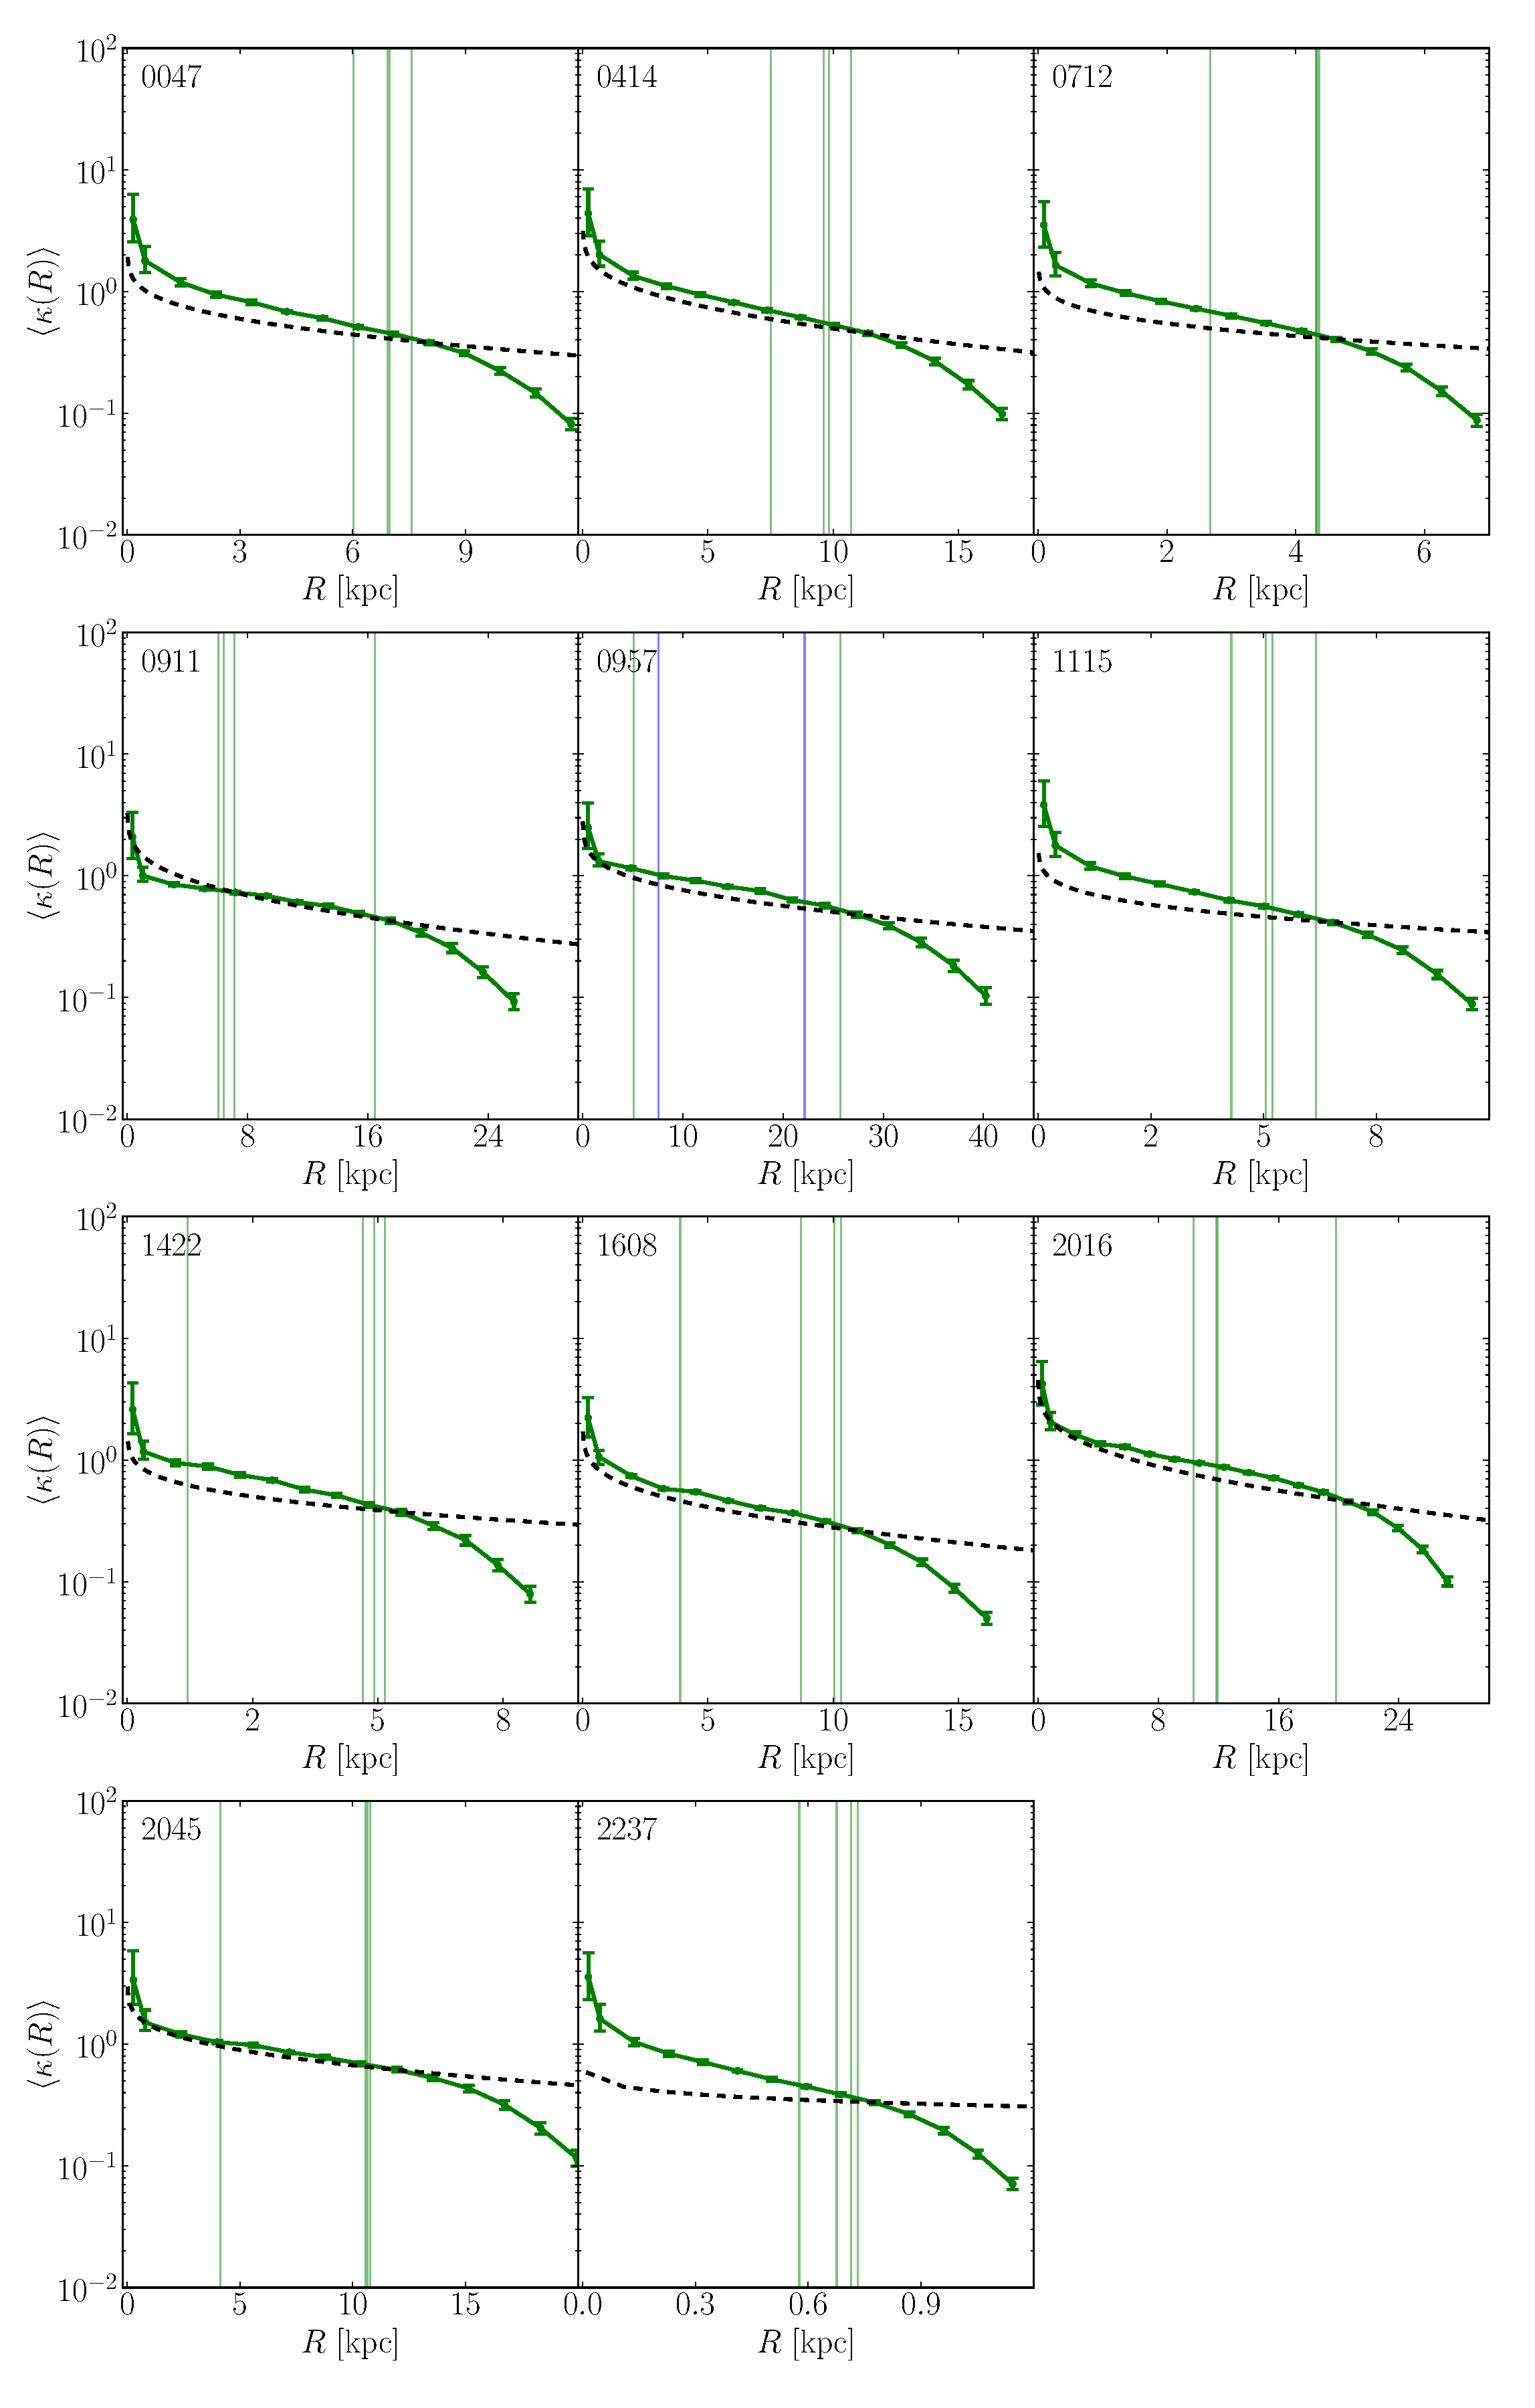
\includegraphics[width=.75\linewidth]{Figures/kappaplot.pdf}
  \caption[width=\linewidth]{Azimuthally averaged convergence $\langle\kappa\rangle$ within radii $R$ of the dark matter distribution. The vertical lines denote the radial distances of the source images from the centre of the lens galaxies. We note that in the case of \textit{0957}, there are two lensed components of the source galaxy. Thus, the green resp. blue vertical lines correspond to the images of the respective components. The green curves show the contributions by the dark matter in the strong lens galaxies as reconstructed by \Glass. The dashed black lines show the corresponding profiles for dark matter halos that follow a NFW density profile. The parameters in the NFW distribution are calibrated in order for the values of the derived convergences $\langle\kappa\rangle$ to match the correspnding values of the reconstructed profiles at one pixel past the last image radius.}
  \label{fig:kappaplot}
\end{figure*}

\begin{figure*}
  \centering
  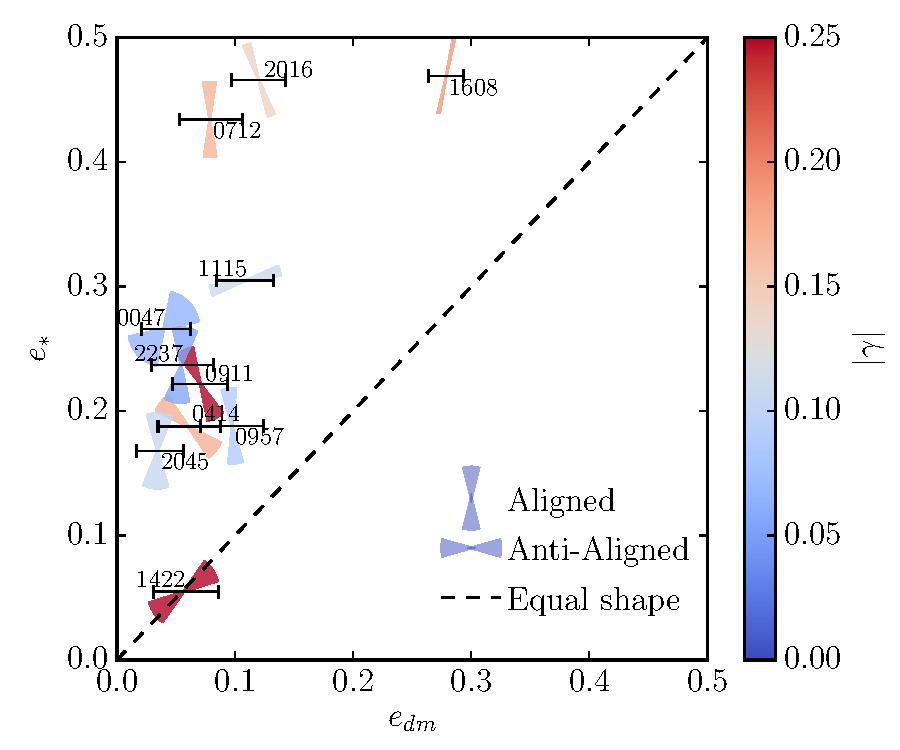
\includegraphics[width=\linewidth]{Figures/wedges_shears.pdf}
  \caption[width=\linewidth]{The reconstructed lens galaxies are displayed according to the reconstructed total shapes of the dark matter halos $s_{dm}$ and the stellar components $s_{*}$. The wedges show the alignment of the semi-major axes of the components. In case of alignment of the respective semi-major axes (Aligned), the wedges are vertical. In case of alignment of the semi-major with the semi-minor axis (Anti-Aligned), the wedges are horizontal. The opening angle of each wedge displays the statistical error in the shape estimate of the dark matter halos. Both the uncertainties in the alignment and the ellipticity of the dark matter distribution denote the ranges $68\%$ of all the mass models of the ensemble of solutions lie within. The lens galaxies are additionally color-coded in terms of the required external shear in reconstructing the mass distribution. The right panel shows the region in the left panel denoted by a dashed rectangle in greater detail.}
  \label{fig:wedgesall}
\end{figure*}

\begin{table*}
  \begin{center}
    \begin{tabular}{l | l l l l l l l l l}
      Lens & $s_{*}$ & $s_{dm}$ & $\Delta\theta$ [$^{\circ}$] & $e_{*}$ & $e_{dm}$ & $e_{dm}/e_{*}$ & $f_h$ & $|\gamma|$ & $\theta_{g}$ [$^{\circ}$] \\ \hline
      % 0047 & 0.27 & 0.04$\pm$0.02 & 0.15 & 0.02$\pm$0.01 & 0.13$\pm$0.07 & 0.10$\pm$0.07 & 0.07$\pm$0.01 & 120$\pm$5 \\
      % 0414 & 0.19 & 0.06$\pm$0.03 & 0.10 & 0.03$\pm$0.01 & 0.30$\pm$0.14 & 0.20$\pm$0.11 & 0.17$\pm$0.02 & 166$\pm$4 \\
      % 0712 & 0.43 & 0.08$\pm$0.03 & 0.28 & 0.04$\pm$0.01 & 0.15$\pm$0.05 & 0.15$\pm$0.05 & 0.17$\pm$0.01 & 141$\pm$3 \\
      % 0911 & 0.22 & 0.07$\pm$0.02 & 0.12 & 0.04$\pm$0.01 & 0.29$\pm$0.10 & 0.27$\pm$0.10 & 0.28$\pm$0.02 & 99$\pm$2 \\
      % 0957 & 0.19 & 0.10$\pm$0.03 & 0.10 & 0.05$\pm$0.01 & 0.49$\pm$0.14 & 0.49$\pm$0.14 & 0.09$\pm$0.03 & 159$\pm$8 \\
      % 1115 & 0.30 & 0.11$\pm$0.02 & 0.18 & 0.06$\pm$0.01 & 0.32$\pm$0.07 & 0.08$\pm$0.04 & 0.11$\pm$0.01 & 154$\pm$3 \\
      % 1422 & 0.05 & 0.06$\pm$0.03 & 0.03 & 0.03$\pm$0.01 & 1.03$\pm$0.51 & 0.64$\pm$0.41 & 0.26$\pm$0.01 & 39$\pm$1 \\
      % 1608 & 0.47 & 0.28$\pm$0.01 & 0.31 & 0.16$\pm$0.01 & 0.53$\pm$0.03 & 0.52$\pm$0.03 & 0.19$\pm$0.01 & 145$\pm$2 \\
      % 2016 & 0.47 & 0.12$\pm$0.02 & 0.30 & 0.06$\pm$0.01 & 0.21$\pm$0.04 & 0.20$\pm$0.04 & 0.14$\pm$0.02 & 42$\pm$4 \\
      % 2045 & 0.17 & 0.03$\pm$0.02 & 0.09 & 0.02$\pm$0.01 & 0.19$\pm$0.11 & 0.19$\pm$0.11 & 0.11$\pm$0.02 & 23$\pm$7 \\
      % 2237 & 0.24 & 0.05$\pm$0.03 & 0.13 & 0.03$\pm$0.01 & 0.21$\pm$0.10 & 0.21$\pm$0.10 & 0.06$\pm$0.01 & 159$\pm$4 \\
      0047 & 0.27 & 0.04$\pm$0.02 & -41$\pm$33 & 0.15 & 0.02$\pm$0.01 & 0.13$\pm$0.07 & 0.02$\pm$0.15 & 0.07$\pm$0.00 & 120$\pm$5 \\
      0414 & 0.19 & 0.06$\pm$0.03 & 50$\pm$15 & 0.10 & 0.03$\pm$0.01 & 0.30$\pm$0.14 & -0.05$\pm$0.15 & 0.17$\pm$0.00 & 166$\pm$4 \\
      0712 & 0.43 & 0.08$\pm$0.03 & -0$\pm$10 & 0.28 & 0.04$\pm$0.01 & 0.15$\pm$0.05 & 0.15$\pm$0.05 & 0.17$\pm$0.00 & 141$\pm$3 \\
      0911 & 0.22 & 0.07$\pm$0.02 & 25$\pm$14 & 0.12 & 0.04$\pm$0.01 & 0.29$\pm$0.10 & 0.19$\pm$0.12 & 0.28$\pm$0.00 & 99$\pm$2 \\
      0957 & 0.19 & 0.10$\pm$0.03 & 4$\pm$11 & 0.10 & 0.05$\pm$0.01 & 0.49$\pm$0.14 & 0.49$\pm$0.14 & 0.09$\pm$0.00 & 159$\pm$8 \\
      1115 & 0.30 & 0.11$\pm$0.02 & -75$\pm$7 & 0.18 & 0.06$\pm$0.01 & 0.32$\pm$0.07 & -0.28$\pm$0.08 & 0.11$\pm$0.00 & 154$\pm$3 \\
      1422 & 0.05 & 0.06$\pm$0.03 & -51$\pm$18 & 0.03 & 0.03$\pm$0.01 & 1.03$\pm$0.51 & -0.23$\pm$0.65 & 0.26$\pm$0.00 & 39$\pm$1 \\
      1608 & 0.47 & 0.28$\pm$0.01 & -12$\pm$1 & 0.31 & 0.16$\pm$0.01 & 0.53$\pm$0.03 & 0.48$\pm$0.03 & 0.19$\pm$0.00 & 145$\pm$2 \\
      2016 & 0.47 & 0.12$\pm$0.02 & 20$\pm$6 & 0.30 & 0.06$\pm$0.01 & 0.21$\pm$0.04 & 0.16$\pm$0.04 & 0.14$\pm$0.00 & 42$\pm$4 \\
      2045 & 0.17 & 0.03$\pm$0.02 & -4$\pm$20 & 0.09 & 0.02$\pm$0.01 & 0.19$\pm$0.11 & 0.19$\pm$0.11 & 0.11$\pm$0.00 & 23$\pm$7 \\
      2237 & 0.24 & 0.05$\pm$0.03 & -7$\pm$19 & 0.13 & 0.03$\pm$0.01 & 0.21$\pm$0.10 & 0.20$\pm$0.11 & 0.06$\pm$0.00 & 159$\pm$4 \\
    \end{tabular}
    \caption[width=\linewidth]{The ellipticity values of the stellar and dark matter components of the reconstructed strong lens galaxies and their corresponding ratios. The ellipticities $s_{*}$ and $s_{dm}$ are defined by Eq.~\ref{eq:shapeestimate}, while $e_{*}$ and $e_{dm}$ are converted using $e = (\lambda_1-\lambda_2)/(\lambda_1+\lambda_2)$; $\Delta\theta=\theta_{dm}-\theta_{*}$ refers to the misalignment angle between the distributions of luminous and dark matter; $e_{dm}/e_{*}$ denotes the ratio of the ellipticities of the dark matter relative to the stellar distribution; $f_h=(e_{dm}/e_{*})\cdot\mathrm{cos} 2\Delta\theta$ refers to the ratio of the ellipticity component of the dark matter distribution projected along the stellar distribution; $|\gamma|$ and $\theta_{g}$ denote magnitude and direction of the required external shear in the modeling of the strong lens galaxy.} % $e = \frac{\lambda_1-\lambda_2}{\lambda_1+\lambda_2}$
    \label{tab:ellipratios}
  \end{center}
\end{table*}

\begin{figure*}
  \centering
  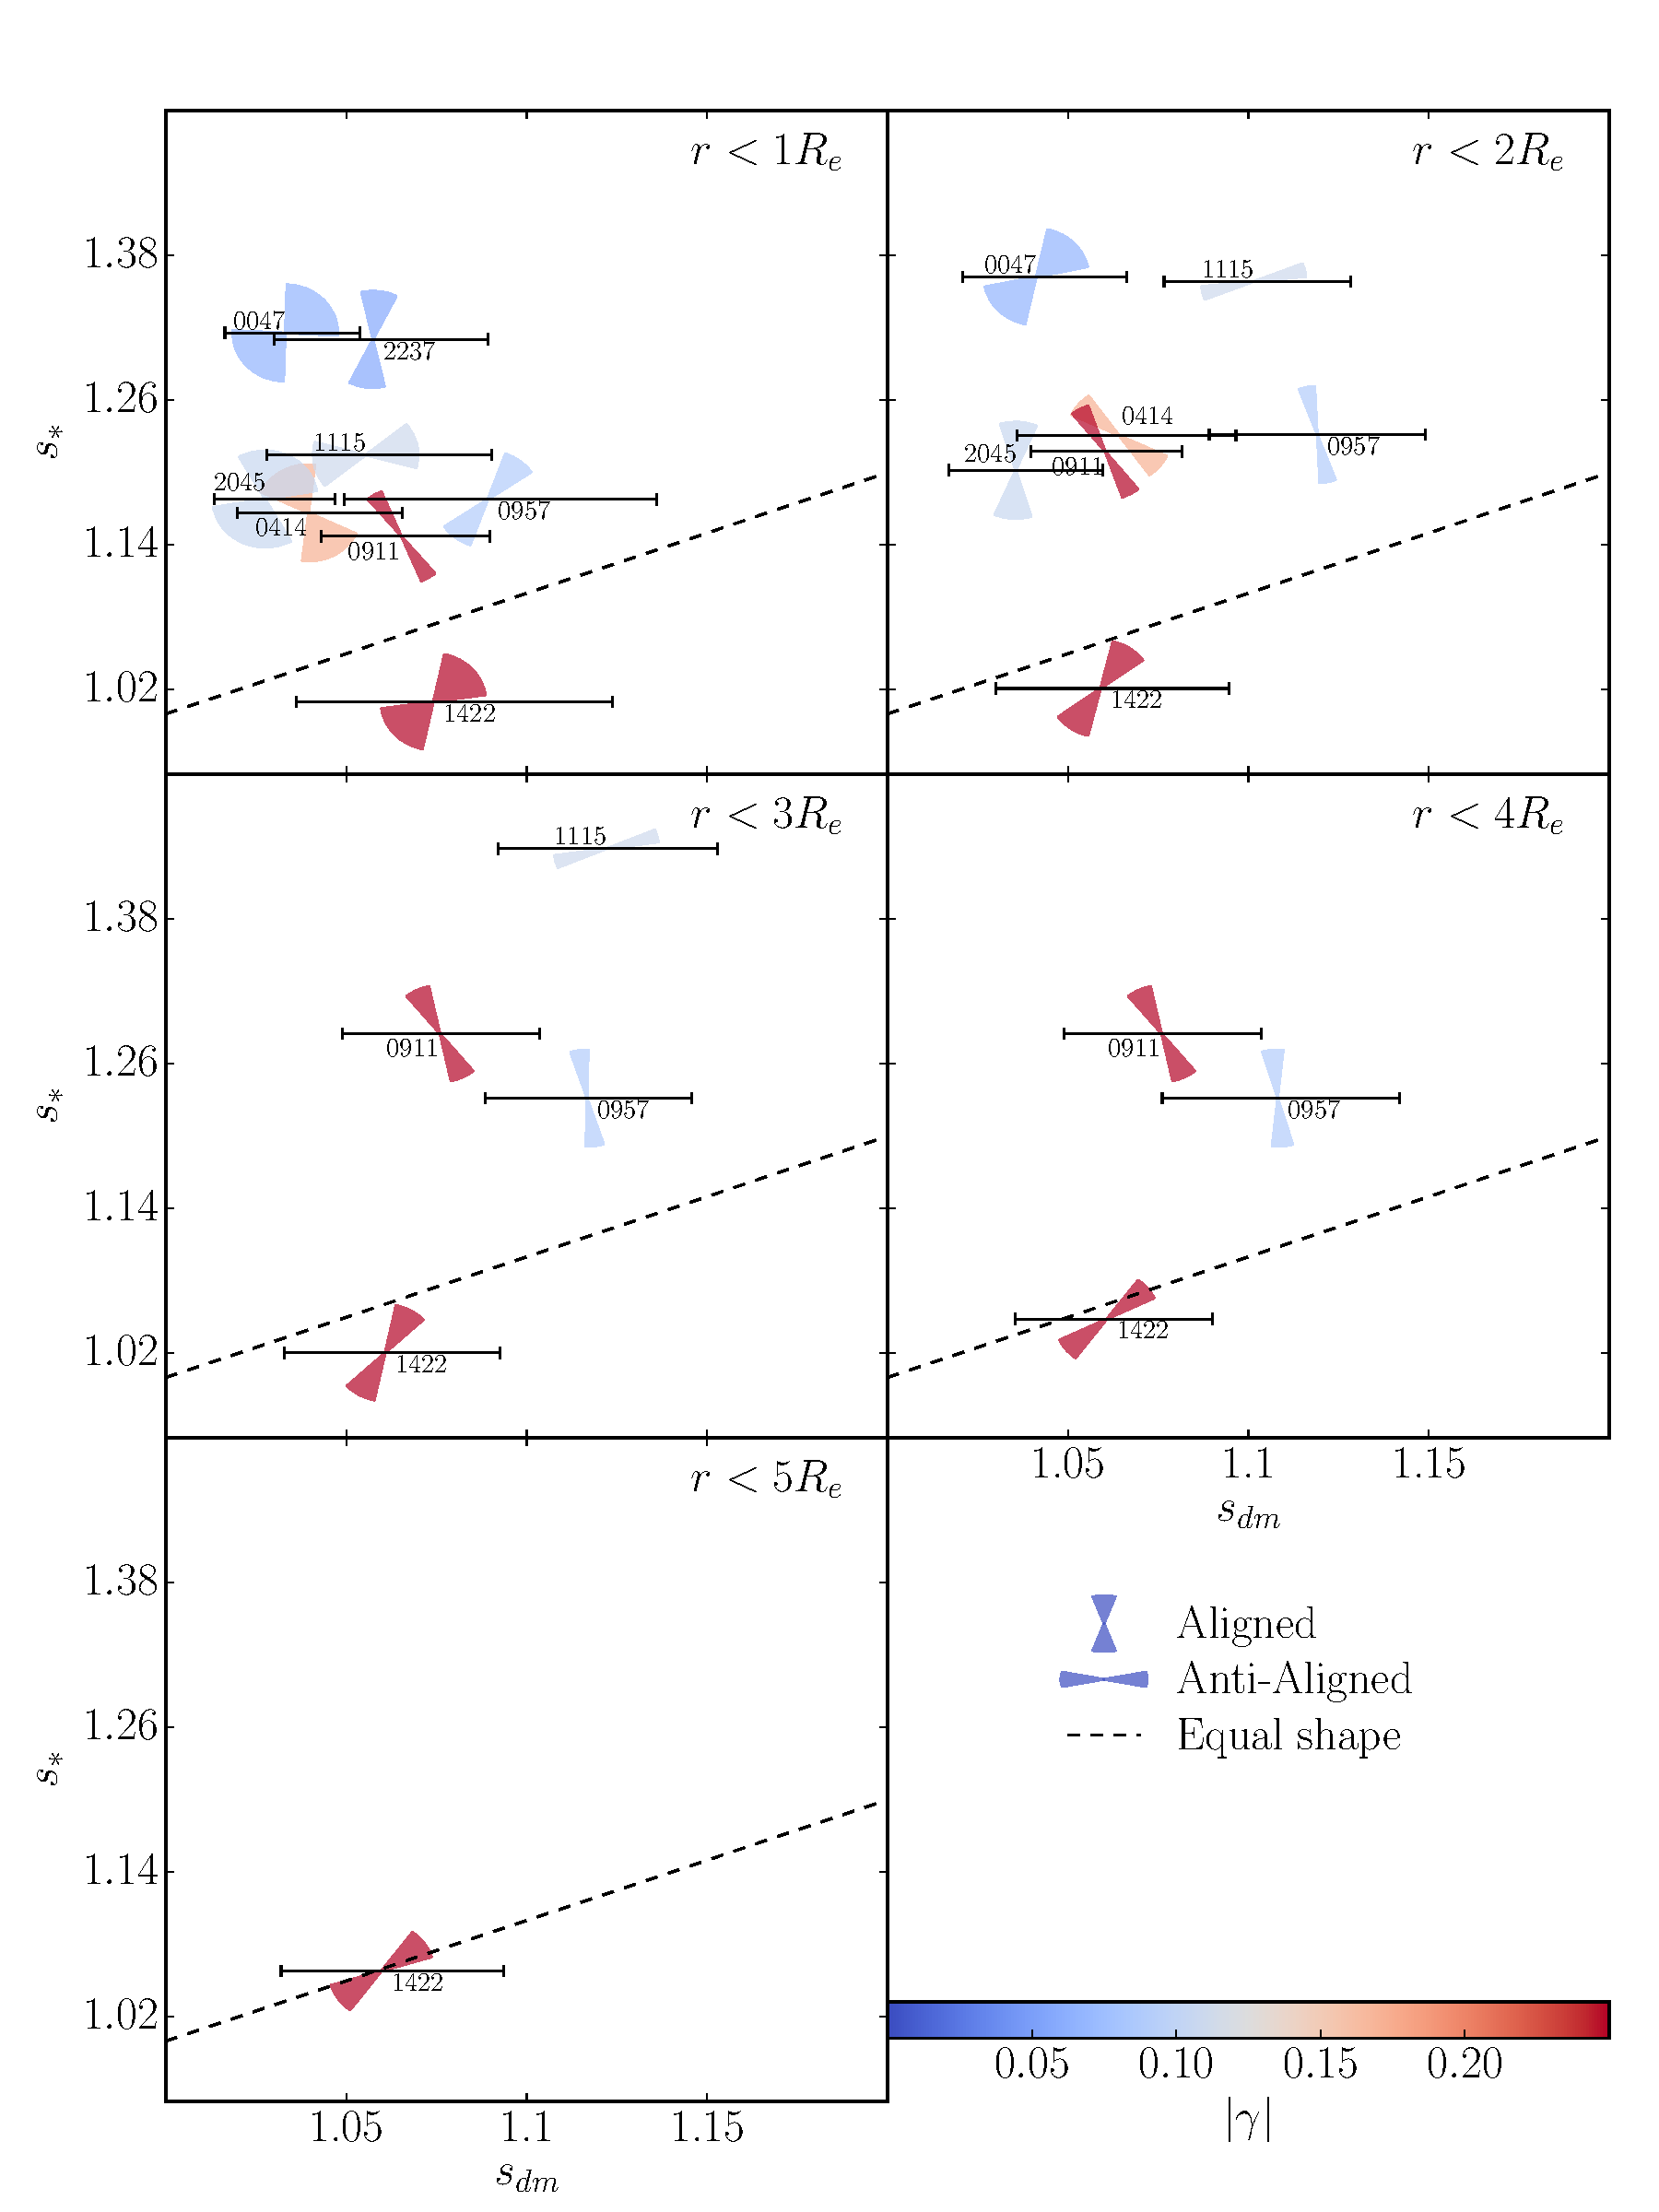
\includegraphics[width=.75\linewidth]{Figures/wedges.pdf}
  \caption[width=\linewidth]{Similar to Figure~\ref{fig:wedgesall}. In each of the subfigures however we only consider pixels within 1, 2, 3, 4, or 5 $R_e$. If the outermost image of a system lies within one of the limiting radii, the system is kept in this panel, but dropped from subsequent panels.}
  \label{fig:wedgesradii}
\end{figure*}

We have applied \Glass\ to the data set described in Section~\ref{sec:data} consisting of 11 lenses. The reconstructed stellar and dark mass maps for each individual lens are given in the Appendix.

\begin{table}
  \begin{center}
    \begin{tabular}{l | l l}
      Lens & $R_{vir}$ [kpc] & $M_{vir} \ [10^{12} \ M_{\odot}]$ \\ \hline
      0047 & 360.7  & 9.98   \\
      0414 & 256.9  & 12.38  \\
      0712 & 446.5  & 15.45  \\
      0911 & 369.1  & 22.66  \\
      0957 & 1053.1 & 175.16 \\
      1115 & 616.8  & 31.06  \\
      1422 & 450.8  & 13.05  \\
      1608 & 317.1  & 9.99   \\
      2016 & 299.3  & 22.14  \\
      2045 & 562.8  & 103.97 \\
      2237 & 1961.0 & 485.26 \\
    \end{tabular}
    \caption[width=\linewidth]{\textbf{[TEMPORARY; IF WE KEEP THIS IN SOME FORM, PROBABLY AS ADDITIONAL COLUMNS TO TABLE~\ref{tab:ellipratios}]}}
    \label{tab:virialmasses}
  \end{center}
\end{table}

\subsection{Radial dark matter profiles}
We compare the profiles of the reconstructed dark matter distributions of the individual strong lens galaxies with Navarro-Frenk-White-profiles \citep[NFW;][]{1996ApJ...462..563N} truncated at the virial radius $R_{vir}$ \citep{2011ApJ...740..102K}
\begin{equation}\label{eq:nfw}
   \frac{\rho(R)}{\rho_{crit}} = \frac{\delta_{c}}{(cR/R_{vir})(1+cR/R_{vir})},
\end{equation}
where $\rho_{crit}$ and $\delta_{c}$ are parameters set by the cosmology considered, $R$ is the radius from the centre, and $c$ is the concentration parameter. The latter is related to $M_{vir}$ \citep{2011ApJ...740..102K}
\begin{equation}\label{eq:concentration}
 \begin{split}
   c(M_{vir}, z) = & c_{0}(z)\left(\frac{M_{vir}}{10^{12}h^{-1}M_{\odot}}\right)^{-0.075} \\ & \times \left[1+\left(\frac{M_{vir}}{M_{0}(z)}\right)^{0.26}\right],
 \end{split}
\end{equation}
where $c_{0}(z)$ and $M_{0}(z)$ are fitting parameters. The relation is constrained at specific redshifts and the parameters are listed in Table 3 of \citet{2011ApJ...740..102K}. For each lens galaxy we choose the parameters at the redshift closest to the lens redshift. 

As the virial radius $R_{vir}$ is related to the virial mass $M_{vir}$ and the concentration parameter $c$, which we however set with Equation~\ref{eq:concentration}, there is only one degree of freedom, $M_{vir}$. We calibrate the mass in order for the derived convergence profiles $\langle\kappa(R)\rangle$ of the reconstructed dark matter distribution and the NFW-profile to match at one pixel past the last image radius.

Figure~\ref{fig:kappaplot} displays the results, while the masses are given in Table~\ref{tab:virialmasses}. \textbf{[HERE SOME COMMENT ON THE MASSES WE HAVE FIT; I'VE INCLUDED THEM TEMPORARILY (!) IN TABLE~\ref{tab:virialmasses} TO DECIDE WHAT WE DO WITH THEM AND HOW WE COMMENT ON THAT SOME OF THESE MASSES ARE RATHER LARGE]}. Except for \textit{0047}, where only the bulge is probed and significant deviations are expected, the profiles agree broadly. There are slight differences in some systems ... \textbf{[HERE WHY WE DON'T WORRY; MAYBE LINK TO FEI LI'S RESULTS?].}

\subsection{Shape and alignment of the dark matter halos}
Figure~\ref{fig:wedgesall} shows our results for the shapes (see Section~\ref{sec:shapemethod}) and alignments of the dark matter and stellar mass distributions. In this Figure, the full distribution up to one pixel past the last-image radius $R_{L}$ is probed. There are several key points to note. Firstly, the reconstructed dark matter distribution of all lenses considered here is rounder than the stellar distribution. Secondly, most lenses lie in the bottom-left corner: the dark matter distributions have typically low eccentricities, while the stellar distributions can be rather elliptical. Thirdly, 3 out of the 11 systems, {\it0712}, {\it2016}, and {\it1608}, stand out due to their larger stellar ellipticity ($s_* > 0.4$). At the same time, they show a very strong alignment between their stellar and dark matter distributions. One of these lenses ({\it1608}) is an known merger of an early-type galaxy with a probable late-type galaxy \citep{2003ApJ...584..100S}. We suggest that the other two systems, {\it0712} and {\it2016}, may also be post-merger systems, explaining their similarities with {\it1608}.

Fourthly, notice that all dark matter and stellar distributions with weak external shear (see the contour bar that displays the shear $\gamma$) are aligned apart from {\it0047} which is almost spherical ($s_{dm}\sim0.05$). By contrast, systems requiring a larger external shear ({\it0414}, {\it0911}, and {\it1422}) can display a sizeable misalignment between the distributions. The latter two systems are located in dense environments (see Table~\ref{tab:lensproperties}) that are likely responsible for these misalignments. As described furthermore in Section~\ref{sec:data}, {\it1422} is a challenging system to model the stellar distribution. {\it0414} has a perturbed along the line of sight contributing to the lensing effect \citep{2011MNRAS.413L..86C}. Besides these three lens systems, one stands out from the rest, however. In {\it1115}, the semi-major axis of the dark matter seems to be aligned with the semi-minor axis of the stellar component; it is the most strongly misaligned (anti-aligned) lens system of all lenses studied here. This may be explained by its external shear ($\gamma \sim 0.1$) emanating from its group environment (see Table \ref{tab:lensproperties}).

We performed tests for the robustness of our shape estimate and its dependence, in particular, on the shear prior. Only two systems, {\it1422} and {\it2045}, reacted to a stricter prior on the external shear $|\gamma|$. {\it1422} requires a rather large external shear ($|\gamma|\sim0.25$). Restricting the range of the allowed external shear values did not affect the misalignment of the dark matter and stellar mass distributions. It did, however, increase the ellipticity of the reconstructed mass distribution: we observed a trade-off between the galaxy's ellipticity and the magnitude of the external shear as might be expected. {\it2045} on the other hand is particularly interesting. Allowing the shear to roam free as for the other lenses, favours an anomalously high shear ($\gamma > 0.5$), with strong misalignment. However, such models also produce spurious extra images along the arc. We find that limiting the maximum shear $|\gamma|$ to 0.1 removes the extra images, though the lens then pushes on its maximum shear prior. We find that the mass map is robust against a stronger shear prior, and does not affect the alignment of the distributions. It produces well-aligned dark matter and stellar distributions. We believe that a strong shear prior for this particular lens is justified by the appearance of spurious extra images if higher shear is allowed.

Figure~\ref{fig:wedgesradii} is similar to Figure~\ref{fig:wedgesall} with the difference that shapes are now averaged within different multiples of $R_e$. There appears to be a trend that the ellipticity of the stellar distribution increases with increasing radius of enclosure. There is potentially a similar trend for the dark matter distribution, although the samples are also consistent with a constant ellipticity. {\it0957}, and to some degree {\it1422}, display, however, some signs of isophotal twist complicating the interpretation (see also Appendix).

\subsection{Consistency with weak lensing estimates}
The ellipticity values $s_{*}$ and $s_{dm}$ shown in Figures~\ref{fig:wedgesall} and \ref{fig:wedgesradii} and the values of the required external shear when reconstructing the lens galaxy are listed in Table~\ref{tab:ellipratios}. Furthermore, the ellipticity $s$ is converted to the ellipticity definition $e=(a-b)/(a+b)$, where $a$ and $b$ are the semi-major and semi-minor axes of the lens galaxy, by applying the relation
\begin{equation}
   e = \frac{s}{2-s}.
\end{equation}

The latter ellipticity definition is commonly used in weak lensing. Especially, it is employed in \citet{2015arXiv150704301S}, a recent study of the shape and alignment of the dark matter halo relative to the distribution of luminous matter. Weak lensing as a probe however cannot constrain $e_{dm}$ directly. Rather, it is sensitive to the ratio $f_{h} = (e_{dm}/e_{*})\cdot\mathrm{cos} 2\Delta\theta$, where $\Delta\theta$ is the misalignment angle between the two distributions, and $e_{dm}\cdot\mathrm{cos} 2\Delta\theta$ is the component of the ellipticity of the dark matter halo projected along the light distribution. In case of perfect alignment and identical shape, $f_{h}$ is equal to 1. In practive however, $f_{h}$ deviates from 1, as among other effects which cannot be disentangled, misalignment of the two distributions and different ellipticities change its value.

In \citet{2015arXiv150704301S} a measurement on CFHTLenS data and on data from the Milennium Simulation \citep{2005Natur.435..629S} with a ray-tracing through by \citet{2009A&A...499...31H} is performed. The constraints in the highest mass bin of early-type galaxies ($\mathrm{log_{10}}M_{*}>11$) on CFHTLenS data are $f_{h}=-0.04^{+0.25}_{-0.25}$. On the simulated data, including cosmic shear and realistic misalignments between the luminous and the dark matter, the constraints in the highest mass bin and for redshifts $0.4<z<0.6$ are $f_{h} = 0.359^{+0.011}_{-0.010}$. Due to a narrower intrinsic ellipticity distribution in the simulated data however, the latter constraints need to be corrected for with a factor $\approx 1/1.46$. Our results are broadly consistent with both constraints, with the exception of the galaxy merger system \textit{1608} and \textit{1115}. The sample is however not large enough for a quantitative comparison.


\section{Conclusions}\label{sec:conclusions}
We have measured the shape and alignment of the stellar and dark matter distributions in 11 lens systems using a new non-parametric lens tool, \Glass\. We focussed on lenses that have either time delay data or stellar mass maps that contribute significantly to the central potential to determine the projected shape of their dark matter haloes \citep{2014MNRAS.445.2181C}. We measured the shape and alignment using the eigenvalues $\lambda_i$ and eigenvectors of the 2D moment of inertia tensor of the stellar and dark matter distributions, defining a {\it shape parameter} $s = 1 - \lambda_{2}/\lambda_{1}$ ($\lambda_{1} \geq \lambda_{2}$; see Section~\ref{sec:shapemethod}). We averaged $s$ over the range 1-5$R_e$, where $R_e$ is the effective radius of the light profile.

Our key results are as follows:

\begin{itemize}
\item \textbf{[ADD HERE SOMETHING ON THE KAPPA PROFILES?]}

\item We found that the dark matter haloes are rounder than the light distribution over the range $1R_e < R < 5R_e$. As we average over larger radii, the lenses, except the ones with a large stellar ellipticity, become increasingly elliptical in their stellar distributions. The same trend can furthermore be seen for the dark matter, although the data are also consistent with no change in shape. The dark matter haloes are never more elliptical than $s_{dm} = 0.2$, while their stars can extend to $s_* > 0.3$.

\item Three systems have a high stellar ellipticity ($s_* > 0.45$) and correspondingly high alignment between light and dark. One of these -- {\it1608} -- is a known merging pair; we speculate on the other two lens systems ({\it0712} and {\it2016}) being recent post-merger systems as well. 

\item Galaxies with high dark matter ellipticity and weak external shear show strong alignment; those with strong shear ($\gamma \gtrsim 0.1$) can be highly misaligned. This is reassuring since isolated misaligned galaxies are expected to be unstable \citep[e.g.][]{1979ApJ...233..872H,1988A&A...206..269M,2007ApJ...670.1027A,2015arXiv150203429D}.

\item \textbf{[ADD HERE SOMETHING ON THE CONSISTENCY WITH WEAK LENSING RESULTS?]}

\end{itemize}

\textbf{[ADD THE COMMENTED REFERENCES ON MISALIGNMENTS BEING UNSTABLE IN THE .tex-FILE IN A NEW PARAGRAPH]}
%Relevant references for misalignments being unstable: 
%- http://adsabs.harvard.edu/abs/1978MNRAS.183..779B : 1978MNRAS.183..779B
%- http://adsabs.harvard.edu/abs/1981MNRAS.196..455B : 1981MNRAS.196..455B
%- http://adsabs.harvard.edu/abs/1979ApJ...233..872H : 1979ApJ...233..872H
%- http://adsabs.harvard.edu/abs/1984ApJ...276..101S : 1984ApJ...276..101S
%- http://adsabs.harvard.edu/abs/1987A%26A...182..202R : 1987A&A...182..202R
%- http://adsabs.harvard.edu/abs/1988A%26A...206..269M : 1988A&A...206..269M
%- http://adsabs.harvard.edu/abs/2007ApJ...670.1027A : 2007ApJ...670.1027A

Our results provide a new constraint on galaxy formation models that must explain the origin of low eccentricity dark matter haloes (not expected in pure dark-matter-only simulations), and highly misaligned lens systems. A possible remedy is the fact that we constrain 2D projections of the lensing mass and the light distribution integrated along the line of sight. The misalignments we identified also present a new challenge for those alternative gravity theories in which the light is the only source of gravity in a galaxy, where light and dark must necessarily be highly correlated.


\section{Acknowledgements}\label{sec:acknowledgements}
We thank Simon Birrer for useful discussion. JIR would like to acknowledge support from SNF grant PP00P2\_128540/1. DL's research is part of the project GLENCO, funded under the European Seventh Framework Programme, Ideas, Grant Agreement n. 259349.


\bibliographystyle{mn2e}
\bibliography{paper}


\appendix
\section{Reconstructed Lenses}\label{sec:reconstructions}
\begin{table}
  \begin{center}
    \begin{tabular}{l r r r r}
      Lens & A [''] & B [''] & C [''] & D [''] \\ \hline
      0047 & 1.270 & -0.630 & 0.520 & -0.730 \\
           & 0.105 & -0.995 & -1.045 & 0.705 \\
      0414 & -0.472 & -1.061 & -1.1947 & 0.885 \\
           & 1.277 & -0.661 & -0.255 & -0.361 \\
      0712 & -0.013 & 0.795 & 0.747 & -0.391 \\
           & -0.804 & -0.156 & -0.292 & 0.307 \\
      0911 & 2.226 & -0.968 & -0.709 & -0.696 \\
           & 0.278 & -0.105 & -0.507 & 0.439 \\
      0957$^{a}$ & 1.408 & 0.182 & 2.860 & -1.540 \\
           & 5.034 & -1.018 & 3.470 & -0.050 \\
      1115 & 0.355 & -0.909 & -1.093 & 0.717 \\
           & 1.322 & -0.714 & -0.260 & -0.627 \\
      1422 & 1.079 & 0.357 & 0.742 & -0.205 \\
           & -0.095 & 0.973 & 0.656 & -0.147 \\
      1608 & -1.300 & -0.560 & -1.310 & 0.570 \\
           & -0.800 & 1.160 & 0.700 & -0.080 \\
      2016 & -1.735 & 0.335 & 0.437 & 1.268 \\
           & 1.778 & -1.450 & -1.435 & 0.276 \\
      2045 & 1.121 & 1.409 & 1.255 & -0.507 \\
           & 0.824 & 0.035 & 0.576 & -0.183 \\
      2237 & 0.598 & -0.075 & 0.791 & -0.710 \\
           & 0.758 & -0.939 & -0.411 & 0.271 \\
    \end{tabular}
    \caption[width=\linewidth]{The image positions of all the systems are listed in order of arrival time (image A has the shortest arrival time, image D the longest). The positions are relative to the centre of the lens galaxy. The first row contains the RA coordinate, the second the DEC coordinate of the image. \newline $^{a}$ The source lensed by {\it0957} has a second component. Images A and B are a double associated with the main galaxy component, images C and D with the lensed substructure.}
    \label{tab:lenspositions}
  \end{center}
\end{table}

\begin{figure*}
  \centering
  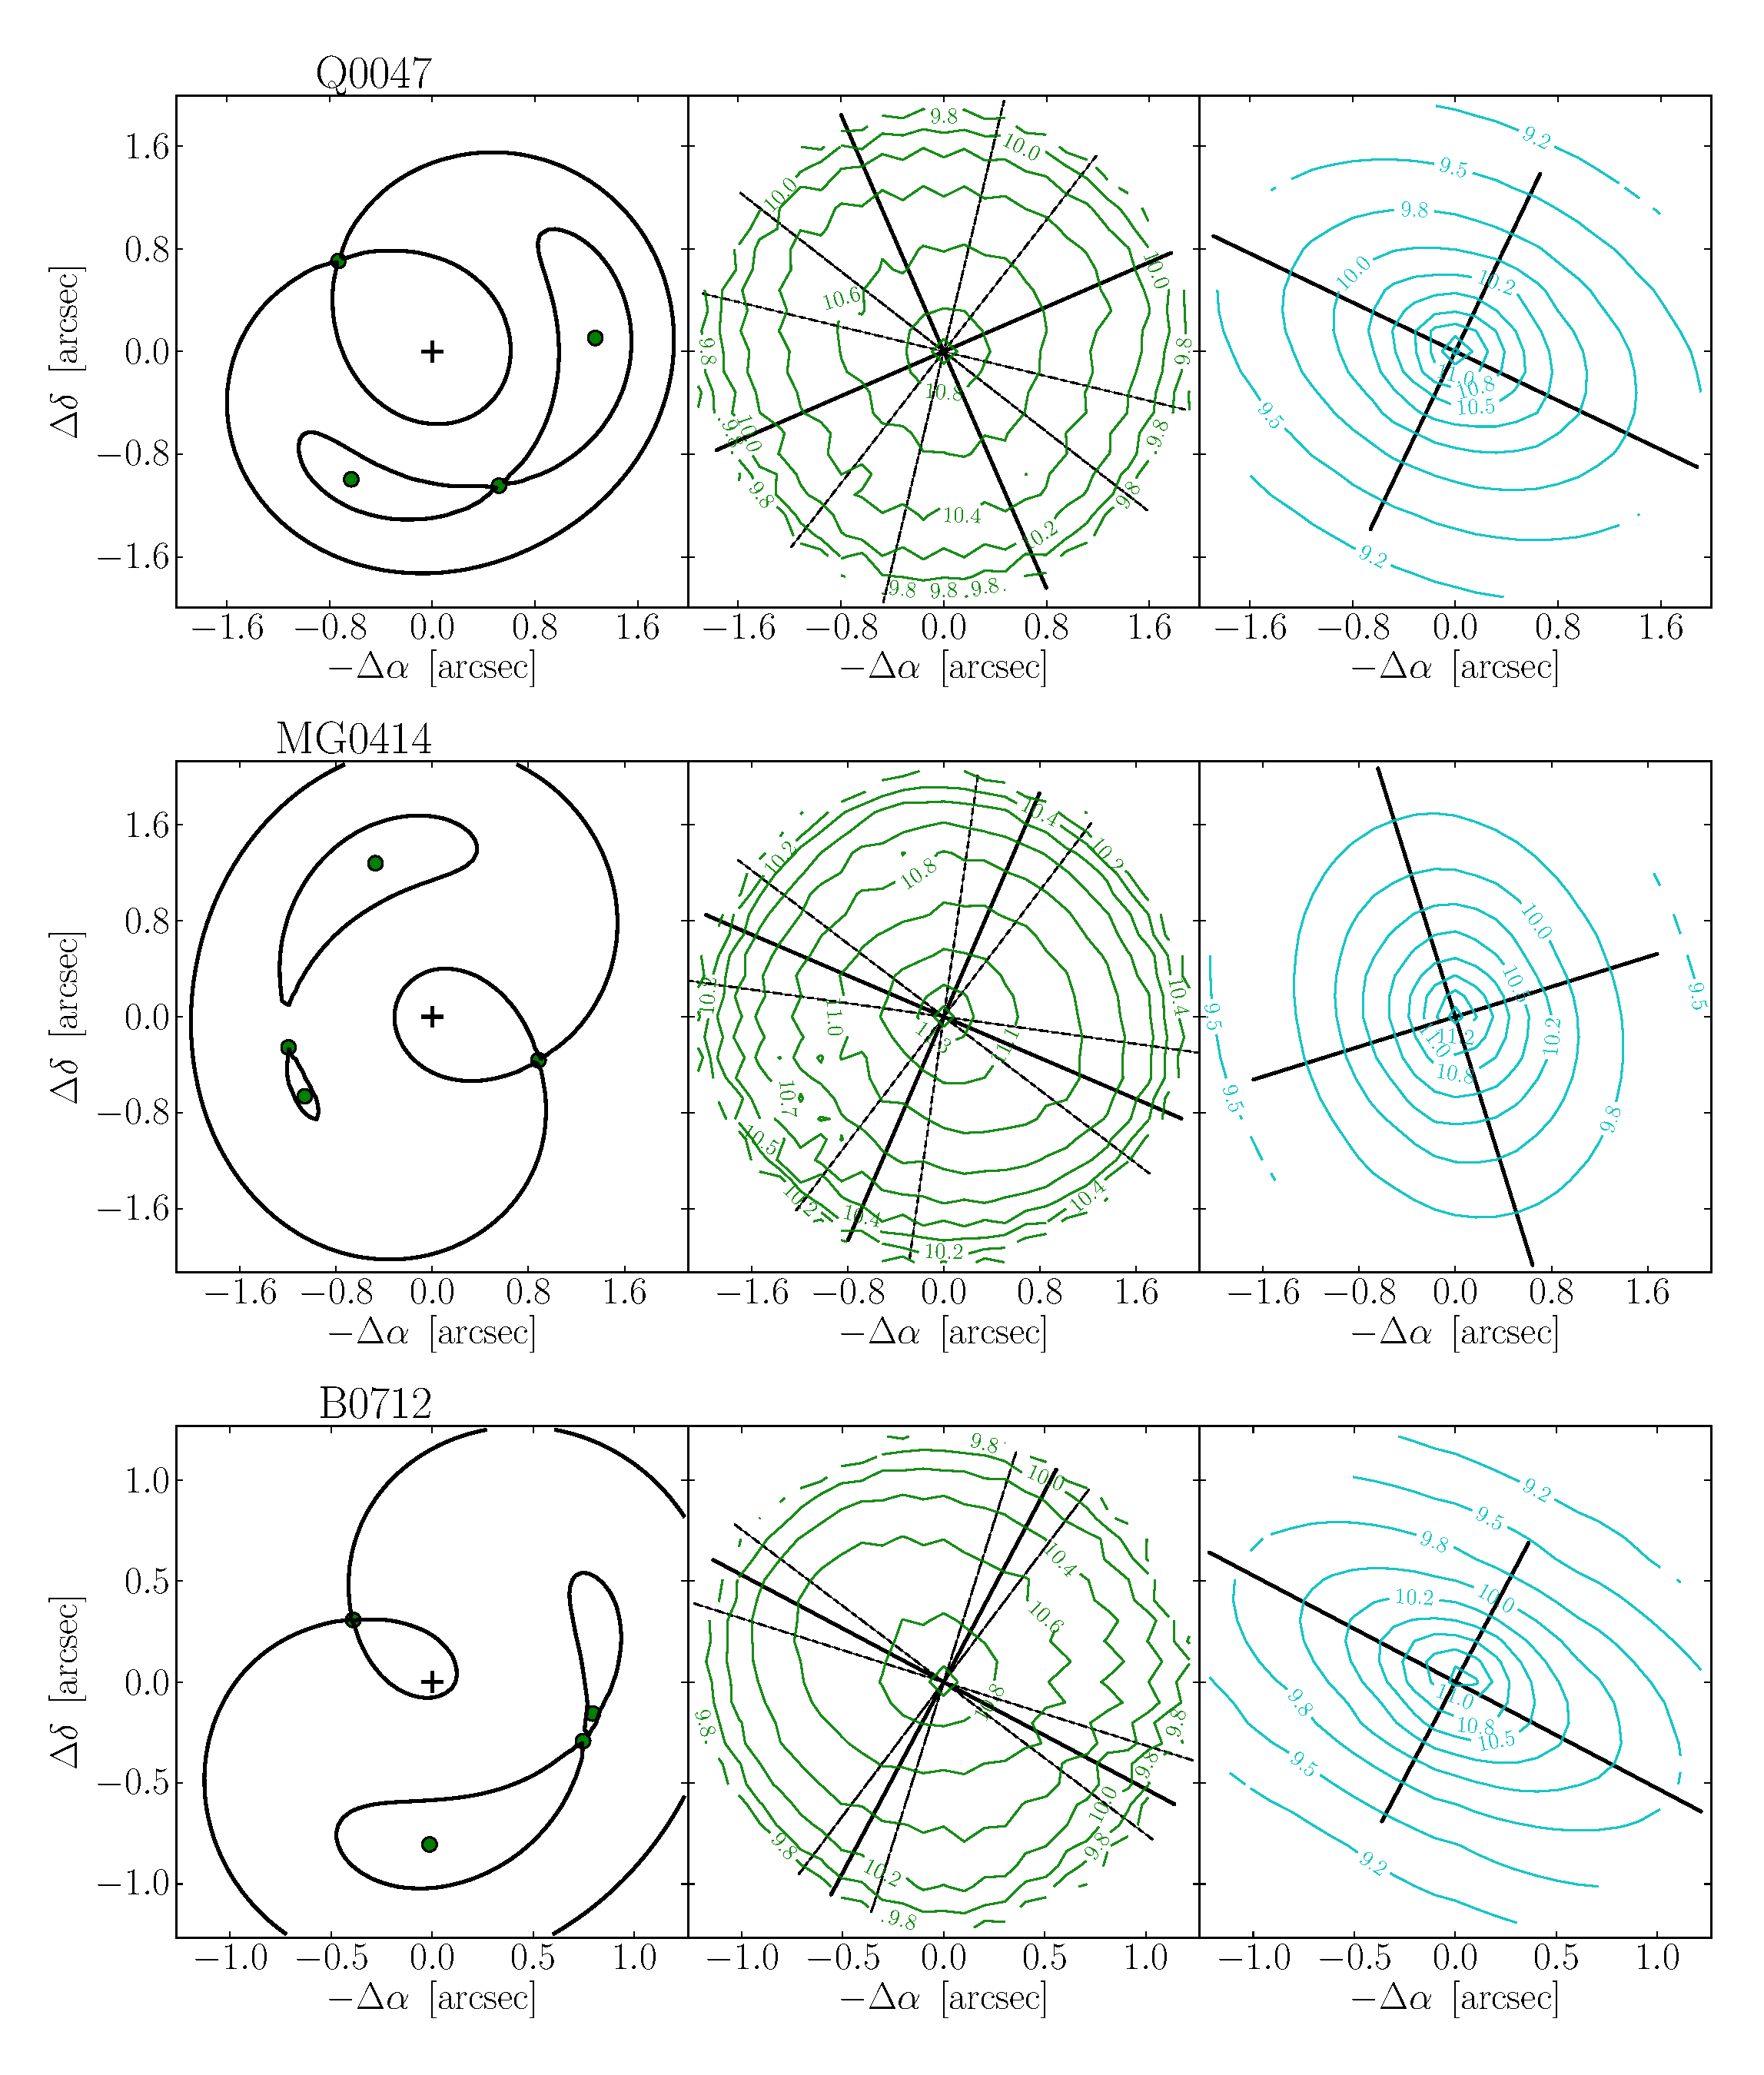
\includegraphics[width=.8\linewidth]{Figures/AllLenses31.pdf}
  \caption[width=.65\linewidth]{The results of our reconstruction of each individual lens galaxy. The panels show, from left to right: the arrival time surface (the images are marked by the green circles); the surface mass density of the dark matter; and the surface mass density of the stars. The solid lines mark the eigenvalues and eigenvectors of the 2D moment of inertia tensor in each case; the dotted lines the 68\% confidence interval of these for the dark matter map.}
  \label{fig:lensreconstruction1}
\end{figure*}

\begin{figure*}
  \centering
  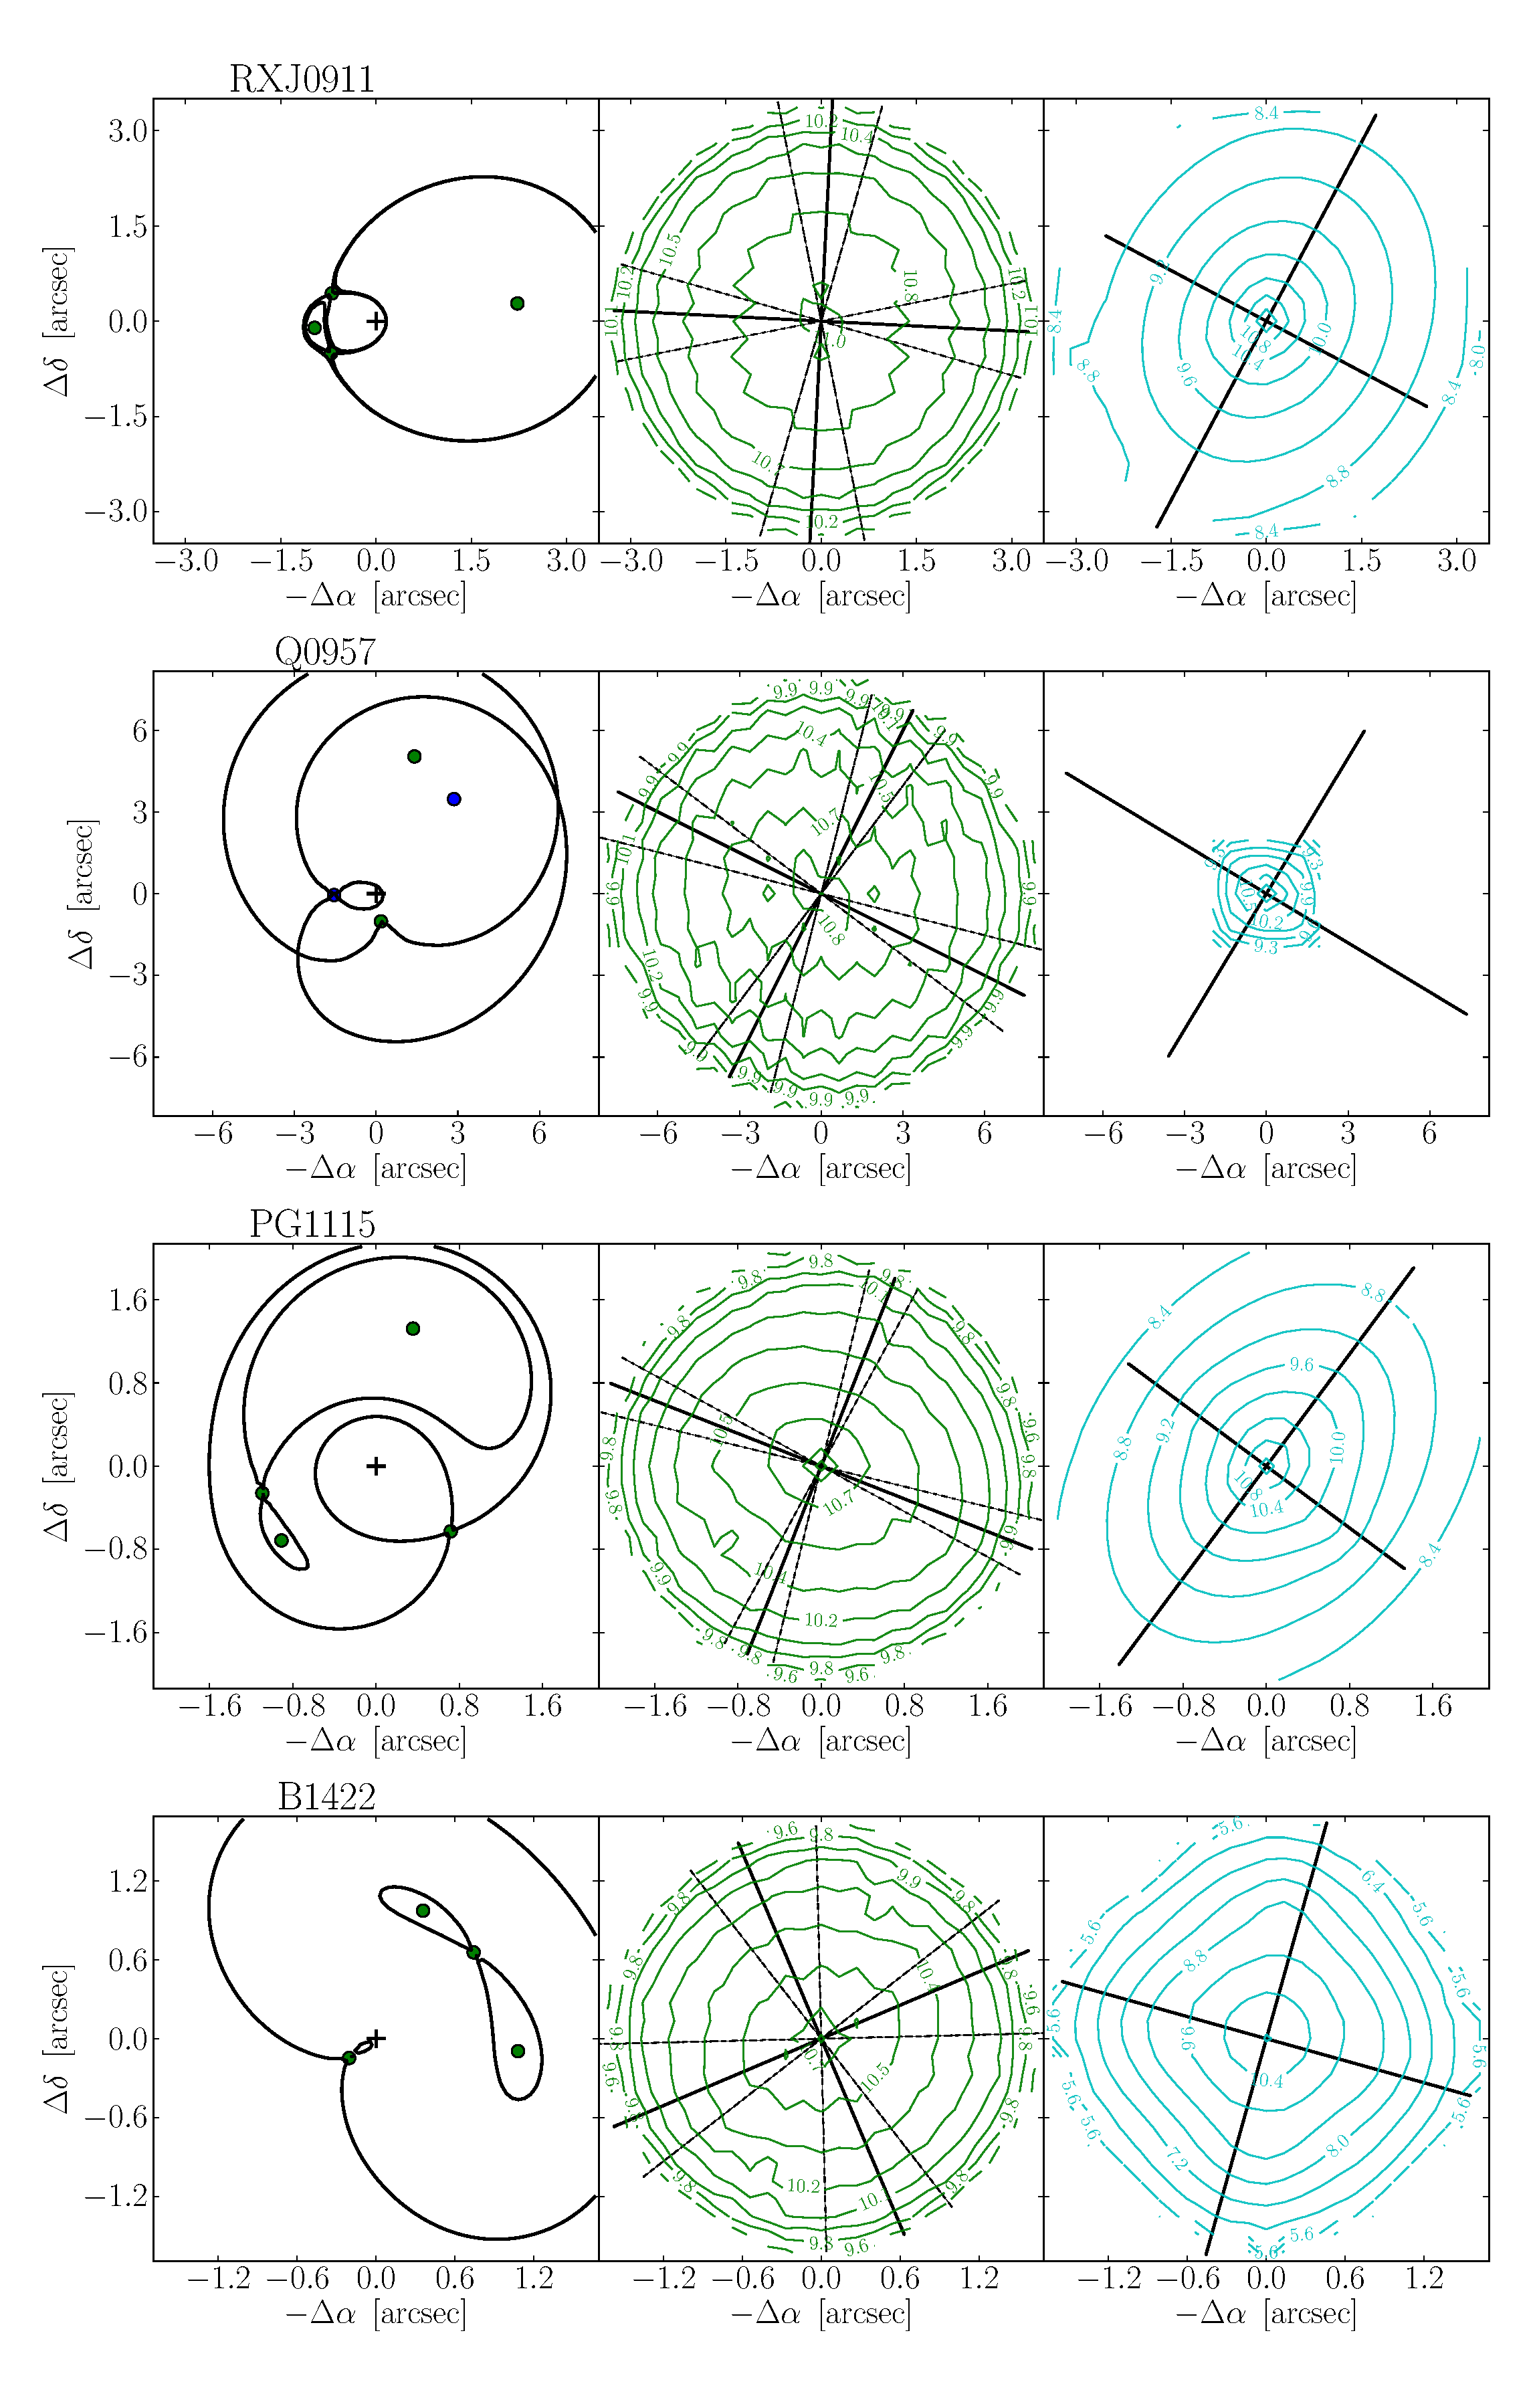
\includegraphics[width=.8\linewidth]{Figures/AllLenses32.pdf}
  \caption[width=.65\linewidth]{The results of our reconstruction of each individual lens galaxy. Lines and symbols are as in Figure \ref{fig:lensreconstruction1}.}
  \label{fig:lensreconstruction2}
\end{figure*}

\begin{figure*}
  \centering
  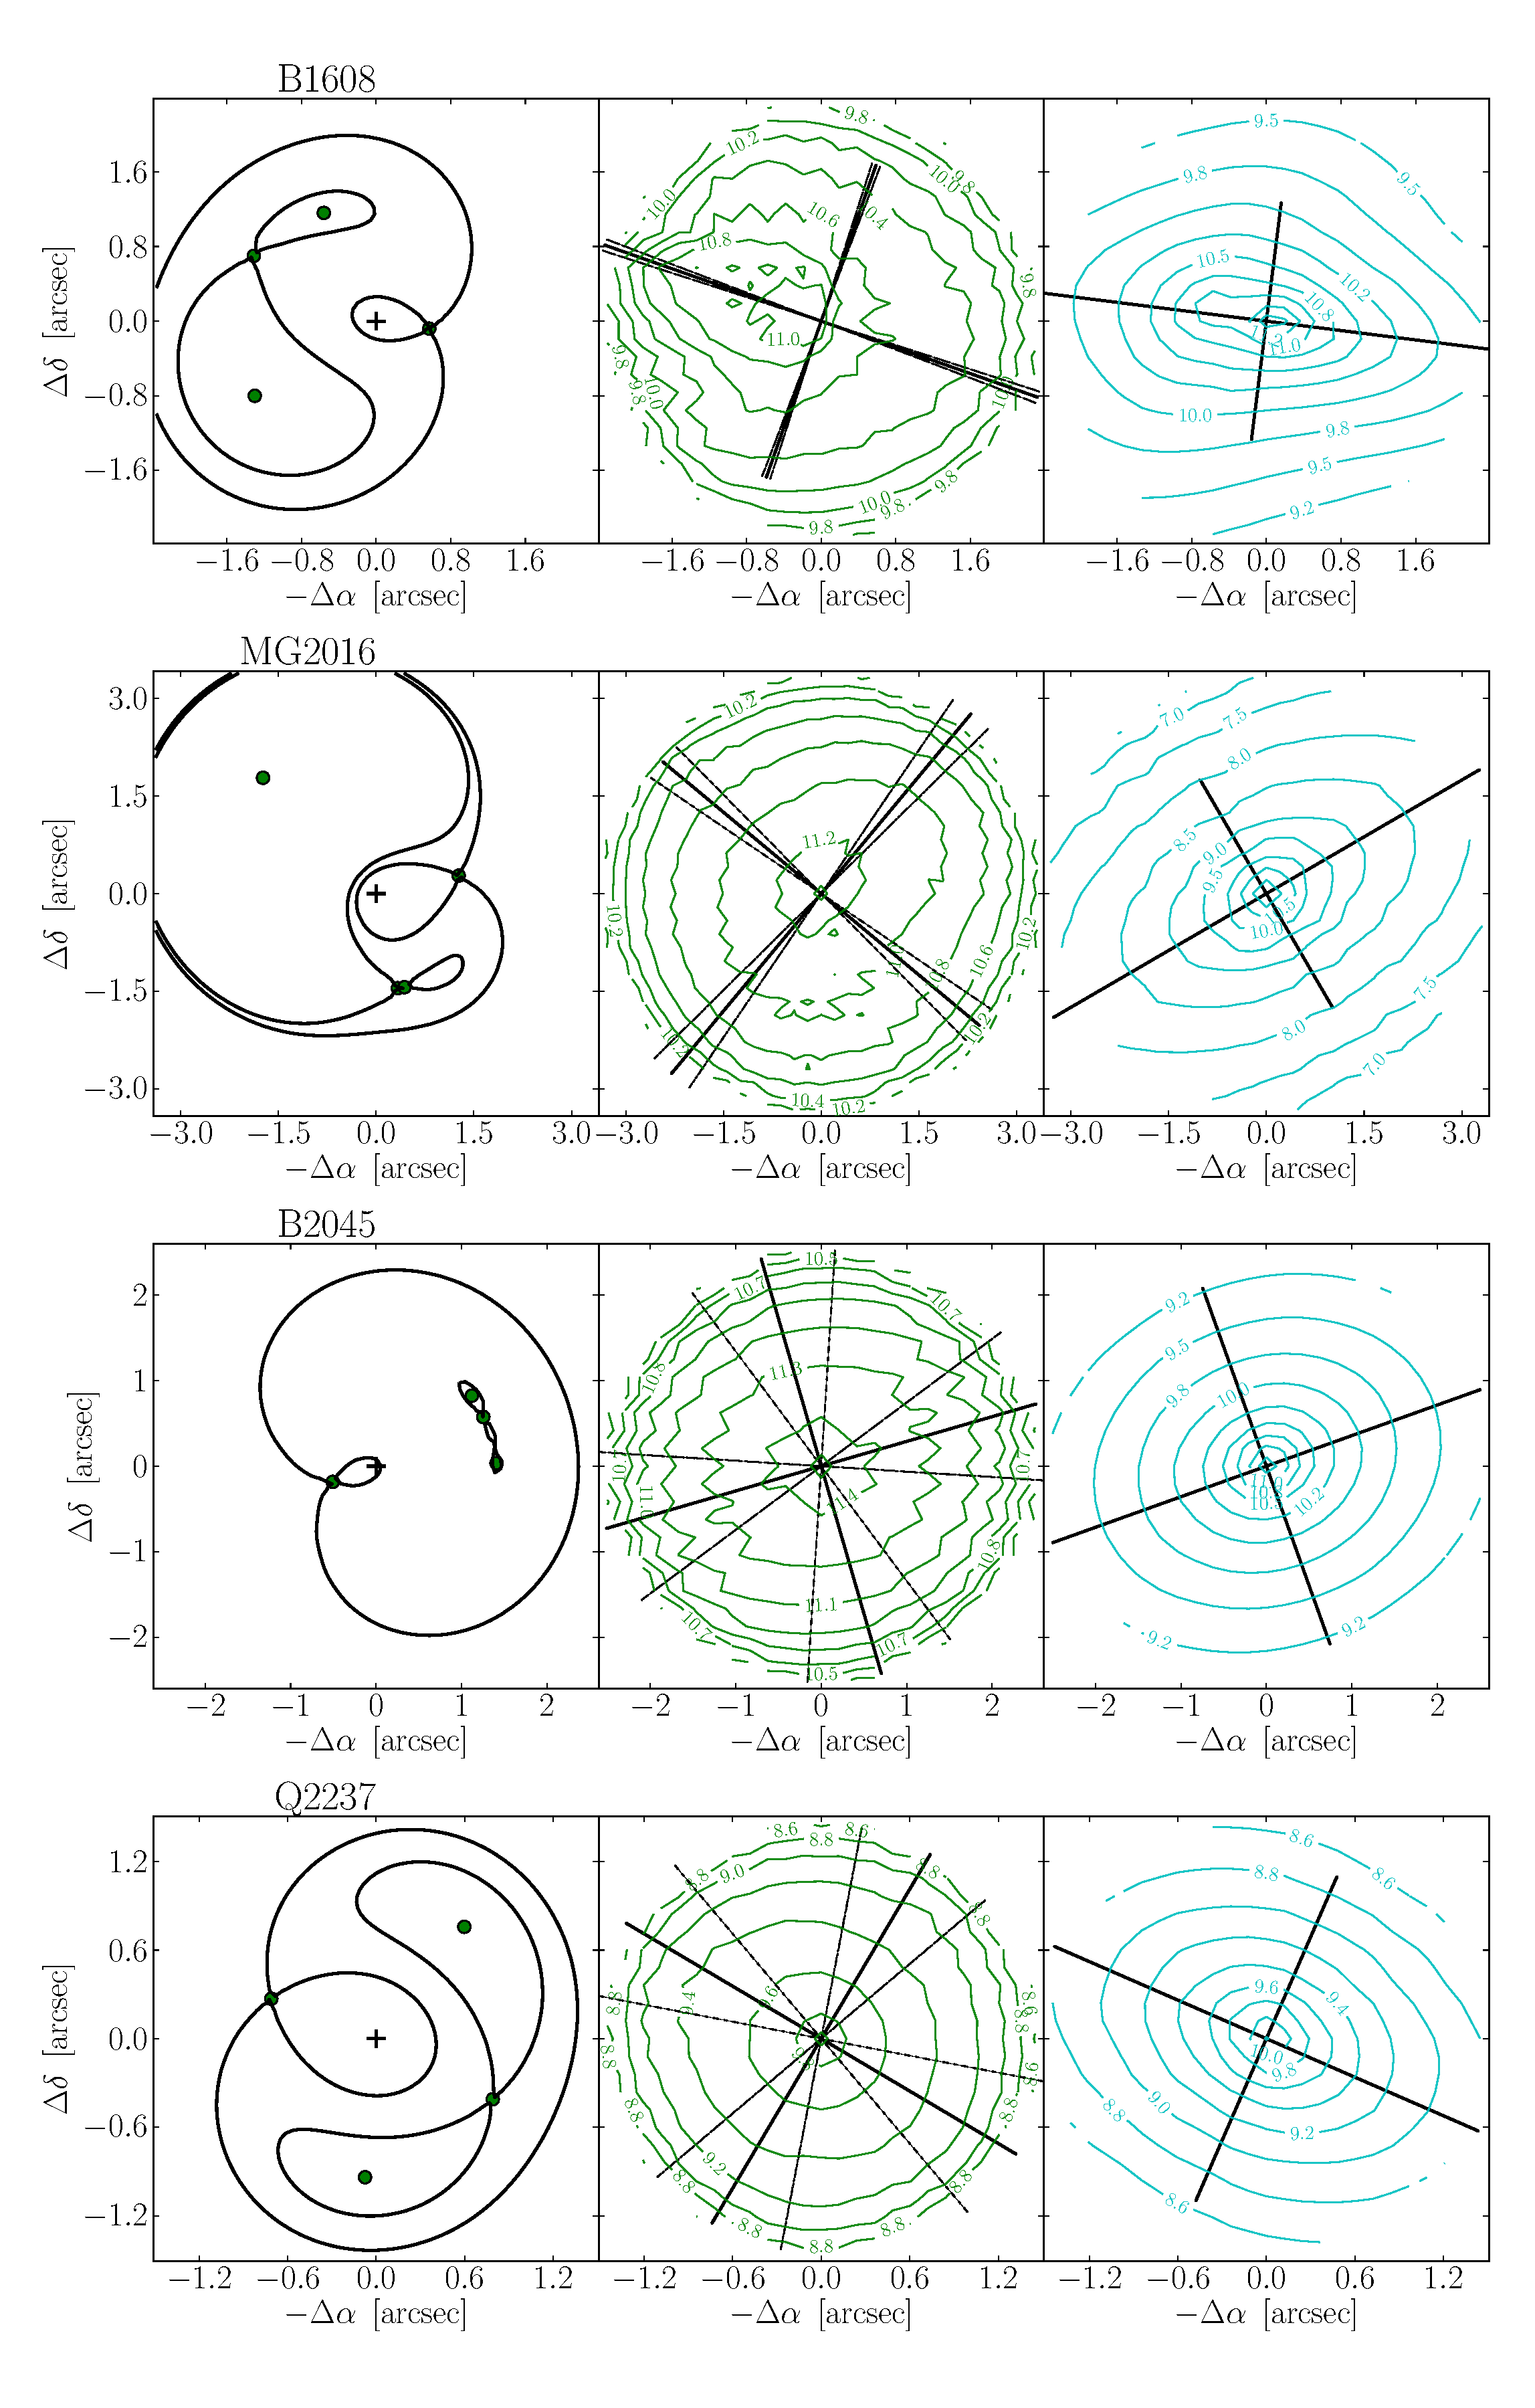
\includegraphics[width=.8\linewidth]{Figures/AllLenses33.pdf}
  \caption[width=.65\linewidth]{The results of our reconstruction of each individual lens galaxy. Lines and symbols are as in Figure \ref{fig:lensreconstruction1}.}
  \label{fig:lensreconstruction3}
\end{figure*}

In this Appendix, we show the results of our lens modelling for each individual lens galaxy (Figures~\ref{fig:lensreconstruction1}-\ref{fig:lensreconstruction3}). The panels show, from left to right: the arrival time surface; the surface mass density of the dark matter; and the surface mass density of the stars. The solid lines mark the eigenvalues and eigenvectors of the 2D moment of inertia tensor in each case; the dotted lines denote the ranges 68\% of all the eigenvectors of the dark matter distribution corresponding to an individual model lie within. Figure \ref{fig:wedgesall} is constructed from the ratio of largest to smallest eigenvalue in each case (to measure the shape parameter $e$), and the angle between the dark matter and stellar major axes. Note that the angular scale is always the same for the dark matter and stellar maps, but varies between the different lenses as marked on the Figure axes.

We note in Figure~\ref{fig:lensreconstruction2}, specifically for {\it0957} and to some degree also {\it1422}, twisting isophotes \citep[e.g.][]{1978ComAp...8...27B}.

\section{Degeneracy between $\theta_{dm}$ and $\theta_{g}$}\label{sec:shearshapedeg}
\begin{figure*}
  \centering
  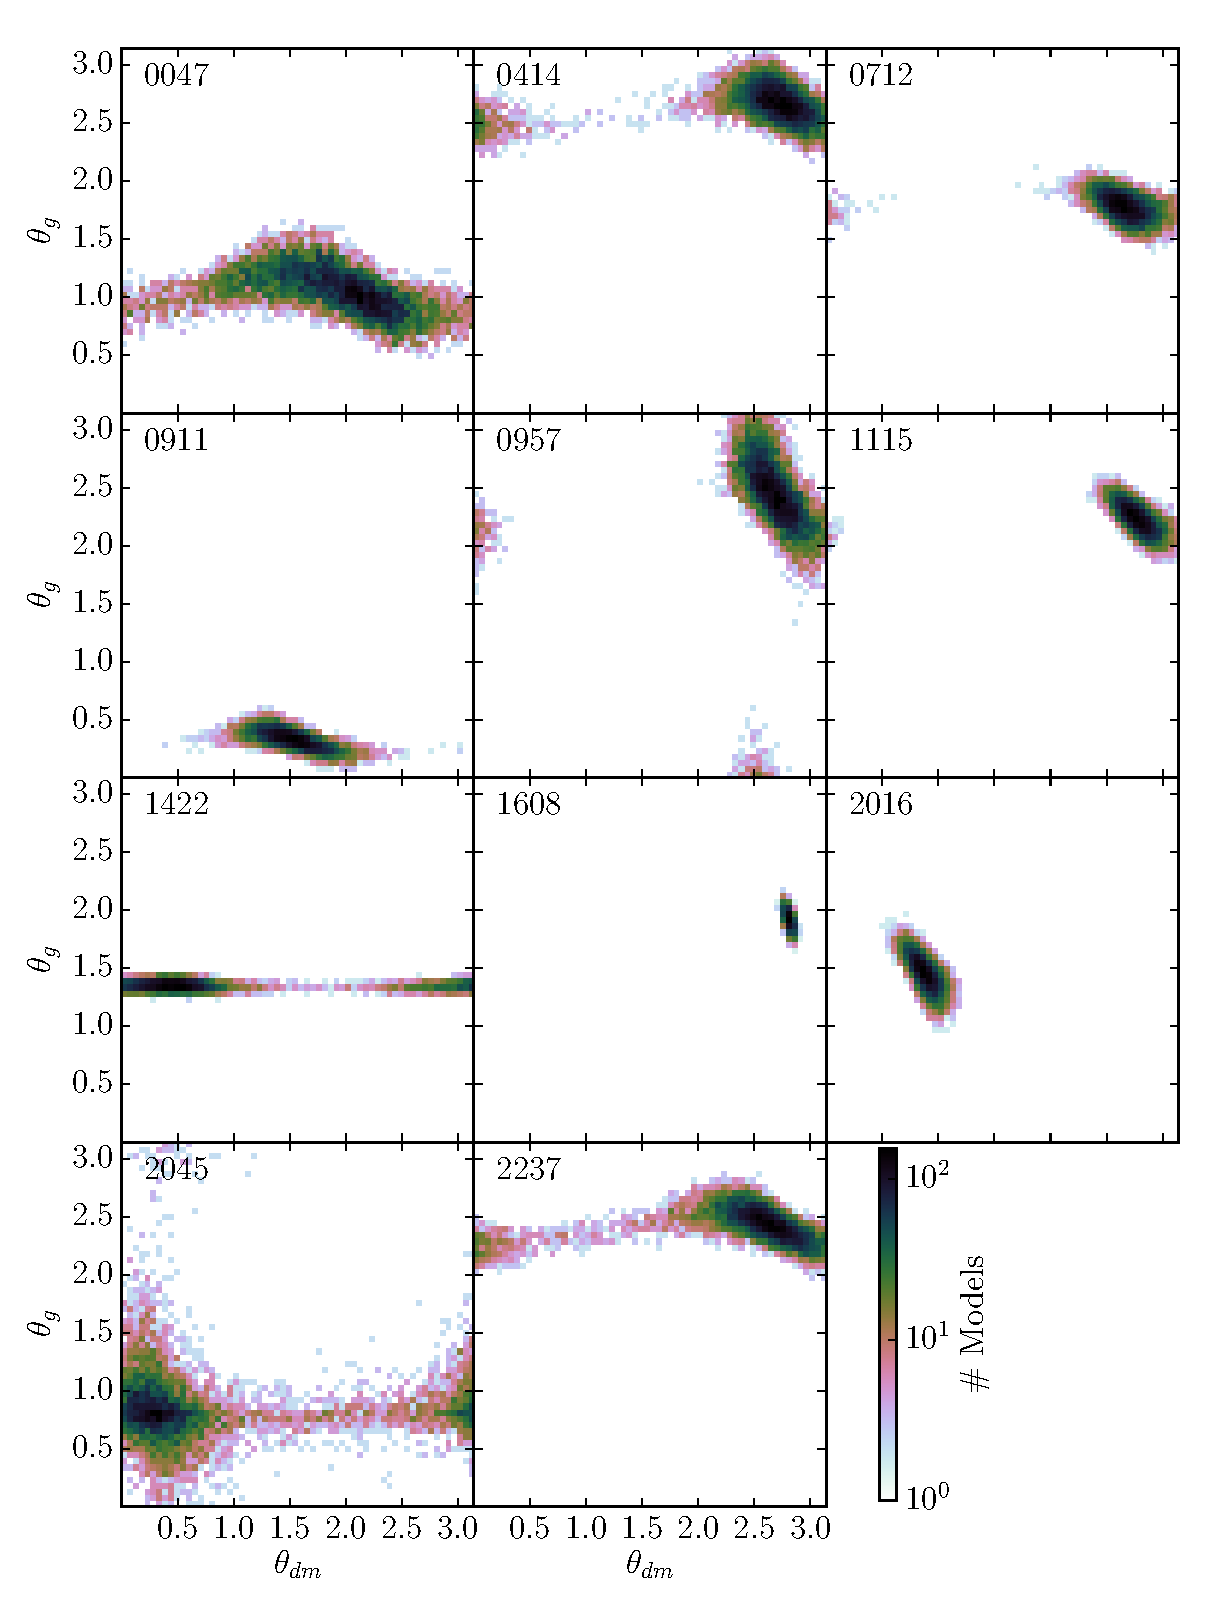
\includegraphics[width=.9\linewidth]{Figures/theta_scatter.pdf}
  \caption[width=\linewidth]{The two-dimensional distribution of the position angles of the dark matter distribution $\theta_{dm}$ and the direction of the required external shear $\theta_{g}$ of each reconstructed mass distribution. The panels display this distribution, which traces the degeneracy of the two parameters, for each reconstructed strong lens galaxy in the ensemble of solutions. Here, the angles are rotated to be measured north through east.}
  \label{fig:thetascatter}
\end{figure*}

Figure~\ref{fig:thetascatter} shows the degeneracy between the position angles of the dark matter halo $\theta_{dm}$ and the external shear $\theta_{g}$ for each strong lens galaxy. We note that the constraints on the direction of the external shear are stronger than the ones on the dark matter distribution \textbf{[INSERT HERE WHY HE THINK THAT IS]}. A slight degeneracy between the angles is evident. However, \textbf{... [WHY THIS IS EXPECTED, AND WHY OUR MISALIGNMENT RESULT STILL HOLDS].}

\end{document}
